\section{Introduction}
Whilst most of this project has focused on improving the interpretation of \acrshort{tds}, this is not the only challenge for widespread utilisation of this type of spectroscopy within the chemical community. As discussed in \Cref{ch:exp_theory}, the experimental apparatus at the University of Leeds for taking these spectra tends to be bulky, complicated to set\nobreakdash-up and come with operational and maintenance challenges. Ti:Sapphire lasers have been the primary method of generating femtosecond \SI{800}{nm} pulses \DIFdelbegin \DIFdel{~}\DIFdelend \cite{Druon2007} but these can suffer from power drift and instability during operation, arising most prominently from temperature fluctuations and resulting in inconsistencies in measurements. Additionally, most sample measurements are performed in a transmission set\nobreakdash-up which necessitates the use of non\nobreakdash-absorbing matrix materials such as \acrshort{ptfe}, owing to strong absorptions above the dynamic ranges of these systems when using pure samples \DIFdelbegin \DIFdel{~}\DIFdelend \cite{Zeitler2016, Smith2011, Murphy2022}. This increases sample preparation complexity and introduces spectral artifacts into the measurements that increase the difficulty of interpretation. Measurements in reflection geometry can be incredibly difficult to align and creating a suitable reference measurement for spectroscopy is also challenging \DIFdelbegin \DIFdel{~}\DIFdelend \cite{Smith2011}. Finally, reflections from both emitters and detectors cause oscillations in the \acrshort{td} that reduce spectral resolution.

With these problems in mind, it was decided to design a new system to address some of these issues. This system is based around the use of a \SI{150}{mW} Toptica Fibre laser. Fibre lasers show more temperature stability than Ti:Sapphire lasers, so there will be less power drift across separate measurements and the consistency of measurements performed using the set\nobreakdash-up will be increased. Initially, the system will be built with the sample in a traditional transmission geometry for ease of alignment and construction but this will be replaced with an \acrfull{atr} accessory \DIFdelbegin \DIFdel{. These }\DIFdelend \DIFaddbegin \DIFadd{which }\DIFaddend are used extensively for mid\nobreakdash-\acrshort{ir} spectroscopy. This accessory will primarily be used to bypass issues with sample permittivity and certain types of spectral artifacts, such as Mie scattering, but eventually will also be used to allow measurements using the full \acrshort{ir} range under identical experimental conditions. All of these improvements should drastically improve the comparability of calculated and experimental spectra and so should increase the accessibility of \acrshort{tds}. 

\section{Investigation into the Effect of Gap Size on the output of a Photoconductive Switch}
Owing to the much lower power output of the fibre laser and the corresponding smaller laser spot size, the larger 100 and \SI{200}{\micro\metre} gap\nobreakdash-size \acrshort{pc} switches, currently in use in System~1 which is described in \Cref{subsec:tdssystems}, would be inefficient for this purpose. These devices would have significant unilluminated portions which would significantly decrease \acrshort{snr}. Whilst some \SI{10}{\micro\metre} devices have been used by this group in the past, it was decided that an investigation into an optimal device gap\nobreakdash-size for lower laser power systems would be beneficial.

The sizes chosen for this study were 5, 10, 20 and \SI{40}{\micro\metre} owing to the expected incident power of 65\nobreakdash-\SI{70}{mW} on the emitter. This is a result of the splitting of the incident pulse into separate beams for emitter and detector and system losses before the emitter. It is estimated that the \SI{5}{\micro\metre} will produce the highest output signal for a given optical power owing to the inverse relationship between gap size and generated signal, but there are other factors that should also be considered. It was decided that the device should be close to saturation at an incident power just above \SI{70}{mW}, which will reduce the magnitude of fluctuations in the device's output resulting from fluctuations in laser power. Saturation, described in \Cref{subsec:pcswitches}, is when increasing incident optical power or applied bias results in a smaller and smaller increase in device output culminating in no increase and eventual damage to the device. This occurs primarily owing to heating in the device and electrical screening from the induced photocurrent. Even with the increased stability of the fibre laser, this is a desirable property. Finally, ease\nobreakdash-of\nobreakdash-alignment should also be considered as the smaller gap\nobreakdash-sizes can be challenging and time\nobreakdash-consuming to optimally align. It should also be considered that when focused onto the emitter, the laser spot has a diameter of approximately 30\nobreakdash--\SI{40}{\micro\metre} which will mean that, with the exception of the \SI{40}{\micro\metre} devices, each gap will not receive 100\% of the incident optical pulse. The desirable device will have the highest output power while still being relatively easy to align and should begin to saturate around \SI{70}{mW}.

\subsection{Fabrication of Photoconductive Switches}
The fabrication of efficient \acrshort{pc} switches for use in the \acrshort{thz} region is non\nobreakdash-trivial and comes with many challenges. The method described below, and shown in \Cref{fig:fabrication}, for the fabrication of these devices onto a sapphire substrate was adapted from Bacon \textit{et. al.} \DIFdelbegin \DIFdel{~}\DIFdelend \cite{Bacon2016}. This method was also used to produce the devices with a \acrshort{si}\nobreakdash-GaAs substrate but without the substrate transfer steps. For all devices, the material used to generate the \acrshort{thz} radiation was \acrshort{lt}\nobreakdash-GaAs and when discussing these devices, they will be differentiated by their substrate material alone.

\begin{figure}[t]
    \centering
    \includegraphics[scale=0.49]{Figures/Misc/SysDev/Fabrication_V2.png}
    \captionsetup{font = footnotesize, justification = centering}
    \caption[A Schematic showing the Fabrication Process for a Photoconductive Switch with a LT-GaAs Substrate]{A schematic showing the fabrication process for a \acrshort{pc} switch with a \acrshort{lt}\nobreakdash-GaAs substrate. This process is also the same for devices with an \acrshort{si}\nobreakdash-GaAs subtrate but without the substrate transfer steps.}
    \label{fig:fabrication}
\end{figure}

A \SI{2}{\micro\metre} thick layer of \acrshort{lt}\nobreakdash-\(GaAs\) was grown, using molecular beam epitaxy at \SI{210}{\celsius}, on a \SI{100}{nm} thick AlAs layer, which was itself grown on a \SI{500}{\micro\metre} thick \acrshort{si}\nobreakdash-GaAs wafer. This is scribed into \SI{2.5}{mm^2} pieces which were placed into a beaker containing acetone and positioned in an ultrasonic bath for \SI{5}{minutes} on 10\% power to avoid damage. This was repeated using isopropyl alcohol (\acrshort{ipa}) to remove any inorganic impurities left on the surface. The final step of the cleaning process involved placing the sample onto a hot plate at \SI{200}{\celsius} for \SI{5}{minutes} which will remove any excess moisture. The sample was then placed in a rapid thermal annealer for \SI{15}{minutes} at \SI{550}{\celsius}. 
The \acrshort{lt}\nobreakdash-GaAs layer on the top of the wafer undergoes epitaxial lift-off where it is removed from the \acrshort{si}\nobreakdash-GaAs substrate. AZ4562 photoresist was applied around the edges of the sample as a barrier as protective wax (Wax W, Apiezon) was melted, using a hotplate at \SI{100}{\celsius}, onto the surface of the \acrshort{lt}\nobreakdash-GaAs. The sample was then placed in a sulphuric etch solution, consisting of \(H_2SO_4:H_2O_2:H_2O\) (1:40:80 by volume), for \SI{5}{minutes} to expose the AlAs layer, and then into a dilute HF solution consisting of HF:\(H_2O\) (1:9 by volume) for \SI{24}{hours} at \SI{4}{\celsius} to remove the AlAs. Once free, the \acrshort{lt}\nobreakdash-GaAs layer, supported by the wax, was transferred onto a clean sapphire substrate and left for approximately one week to allow the excess moisture between the layers to evaporate and bonding to occur. The wax was removed with trichloroethylene and the samples placed in a vacuum oven, for \SI{15}{hours} at \SI{250}{\celsius} and \SI{20}{mbar}, which ensures the removal of any excess moisture and aid further adhesion. After the liftoff and transfer process, devices have been made using both the \acrshort{lt}\nobreakdash-GaAs on substrate and the original \acrshort{lt}\nobreakdash-GaAs on \acrshort{si}\nobreakdash-GaAs and the subsequent fabrication process for both types of devices are identical. 

To perform photolithography on the sample, a bi\nobreakdash-layer resist process is used. This ensures an effective undercut which is vital for the lift\nobreakdash-off process and owing to the S1813 photoresist's poor adhesion with the sapphire substrate. Initially, a primer layer of hexamethyldisilazane is spun onto the surface of sample for \SI{30}{s} at \SI{2000}{rpm}, ensuring coverage of both the \acrshort{lt}\nobreakdash-GaAs and substrate. It is then baked at \SI{200}{\celsius} for \SI{1}{minute} and the first layer of resist (LOR\nobreakdash-3A) is spun on at \SI{2000}{rpm} for \SI{30}{s} which corresponds to an approximate thickness of \SI{0.4}{\micro\metre}. This is baked once again at \SI{200}{\celsius} for \SI{3}{minutes}. Once cooled, a second layer of photoresist (S1813) is spun onto the surface at \SI{4000}{rpm} for \SI{30}{s}, corresponding to a thickness of \SI{1.4}{\micro\metre}, followed by baking at \SI{115}{\celsius} for \SI{4}{minutes}. These were placed into a mask\nobreakdash-aligner (Karl Suss MJB3) where it underwent contact photolithography and was exposed to ultraviolet (\acrshort{uv}) light, centred around \SI{310}{nm}, through an optical mask for \SI{15}{s}. Each sample was then developed in MF319 for \SI{1}{minute}, before being rinsed in water and dried using a dry nitrogen gas. 
To ensure an undercut in the bottom layer of the photoresist, the sample is baked at \SI{180}{\celsius} to crosslink top S1813 layer of photoresist, followed by a further \SI{30}{s} in MF319. The sample could then be positioned upside\nobreakdash-down in a thermal evaporator. Using a low vacuum environment (<~\SI{1.9e-6}{mbar}), approximately \SI{10}{nm} of adhesive Ti and \SI{150}{nm} of Au were evaporated onto the surface of the device. Once completed and cooled, the unexposed photoresist and the excess gold were removed by placing the sample back into a beaker of cyclopentanone for 5 minutes in an ultrasonic bath and dried using dry nitrogen.

As there are many steps and each can suffer from complications, devices fabricated using this method are unlikely to be identical which may explain any variation between nominally identical devices both within the same batch and from different batches.

% Here for figure appearence order
\begin{figure}[h!]
    \centering
    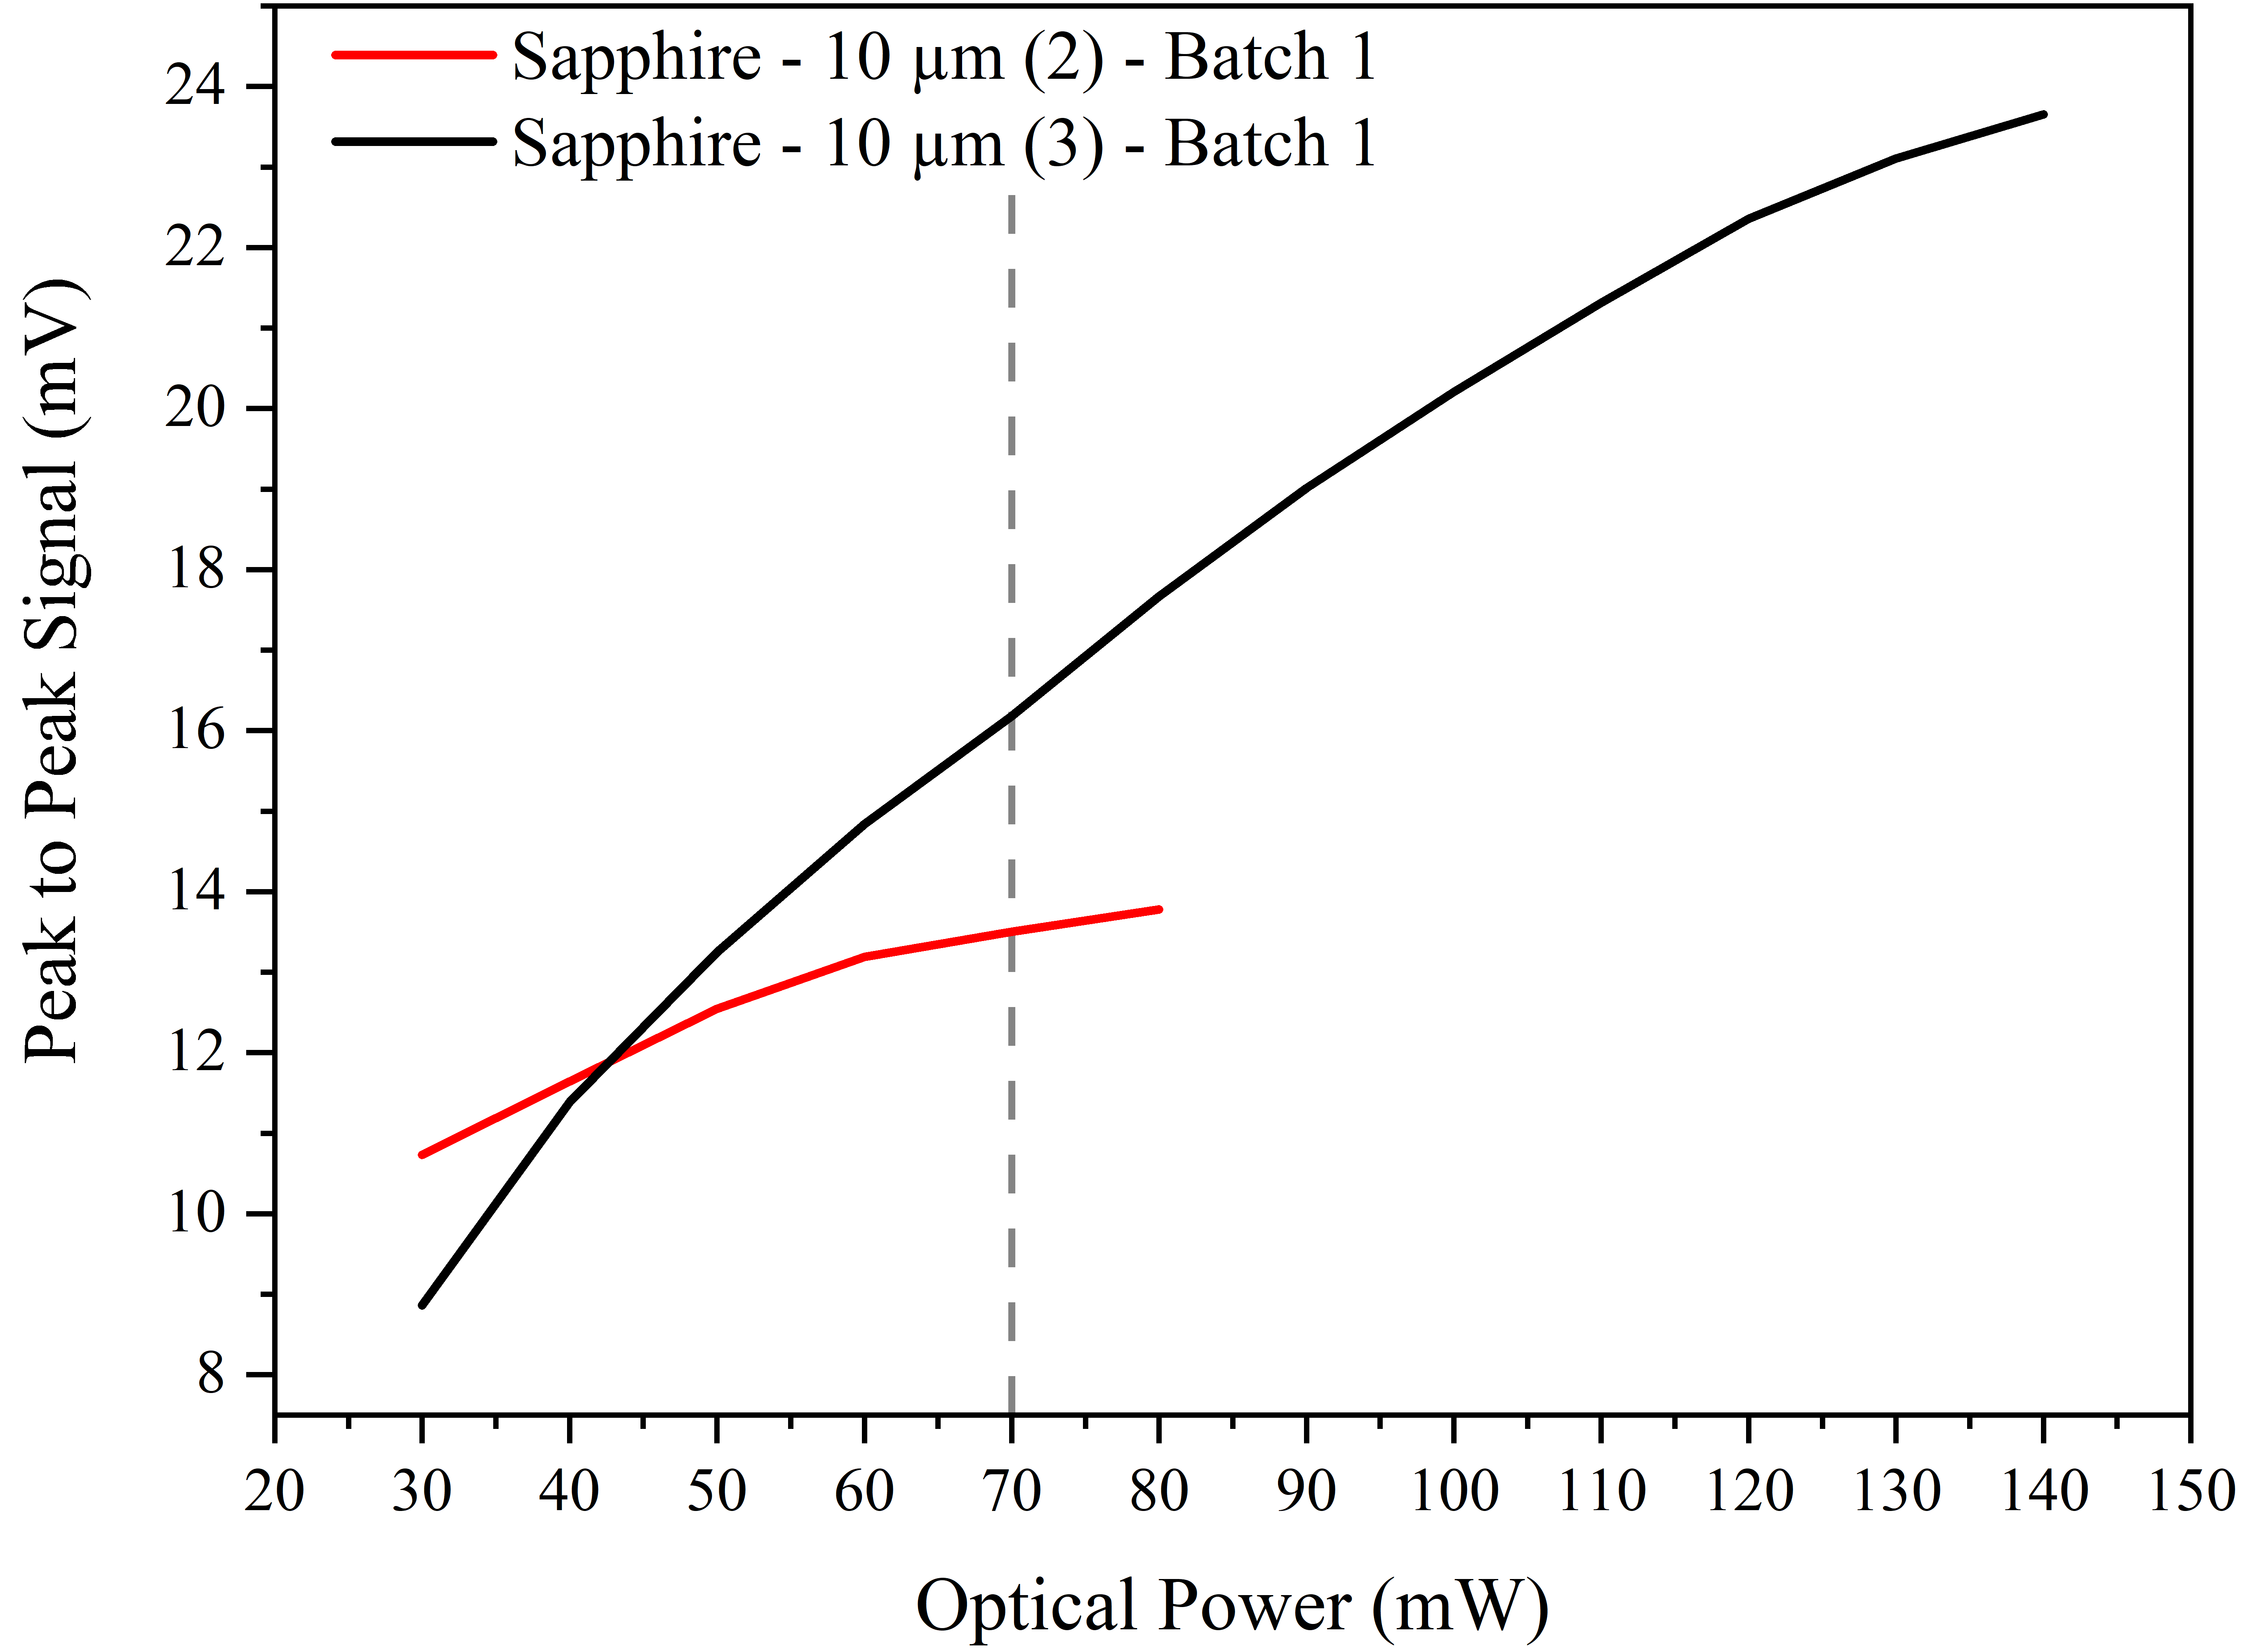
\includegraphics[width=0.6\textwidth]{Figures/Misc/SysDev/Opt10MicronBatch1.png}
    \captionsetup{font = footnotesize, justification = centering}
    \caption[The Peak to Peak Signal Values for Sapphire Batch~1]{The peak to peak signal values for Sapphire Batch~1. There is little agreement between device outputs for the same incident optical power.}
    \label{fig:sapphbatch1}
\end{figure}

\subsection{Testing of Photoconductive Switches}
Using the described method for measuring \acrshort{tds} spectra which is detailed in \Cref{ch:sys_dev}, each device had a bias of \SI{100}{V} applied across it and was initially illuminated with \SI{30}{mW} of incident optical power using an optical attenuator to lower the initial power of the laser. This was then increased in increments of \SI{10}{mW} until the device was considered to be saturated, close to saturation or destroyed which would manifest as a decrease in the slope of the graph of produced signal versus optical power or a sudden drop in signal output. 
\DIFdelbegin \DIFdel{Ideally, the incident field would have been kept constant for the most ideal comparison but maintaining a constant bias simplified the experimental parameters.
}\DIFdelend 

These measurements were performed using a \acrshort{tds} system that will now be referred to as System~2. A mode\nobreakdash-locked Ti:sapphire laser (Maitai DeepSee, Spectra\nobreakdash-Physics) was used to produce \SI{80}{fs} pulses centred at \SI{796}{nm} with a repetition rate of \SI{80}{MHz}. These were directed at the \acrshort{pc} switch being tested and the emissions from this were detected using a \SI{1}{mm} thick ZnTe crystal and a pair of photodiodes which were balanced to \SI{2.8}{V}. The applied bias was modulated using a \SI{7.7}{kHz} square wave. As no sample was present, only one scan was required for each measurement.

Initially, only devices with a sapphire substrate were fabricated but owing to alignment challenges and for a more complete understanding of the underlying processes, devices with an \acrshort{si}\nobreakdash-GaAs substrate were also fabricated from the original wafer and tested. Finally, once the optimum gap size was selected, the chosen \acrshort{pc} switches were tested using the fibre laser utilised in the \acrshort{tds} system under construction which will be referred to as System~3. This will be described in \Cref{sec:fibrelaser}.

\subsection{Results and Discussion}
A set of three \SI{10}{\micro\metre} devices on sapphire substrates had been fabricated previously and these were tested first. One of these was destroyed during alignment but the results from the remaining devices are shown in \Cref{fig:sapphbatch1}. This set of devices will be subsequently referred to as Sapphire Batch~1. The dotted line on each graph of peak\nobreakdash-to\nobreakdash-peak signal versus incident optical power is at \SI{70}{mW} which is the maximum incident optical power from the fibre laser. The desired device will begin to saturate on or just after this line. As these devices should be identical, so should their output signal when illuminated with the same incident optical fluence but in this case, the outputs of each device vary considerably. Additionally, they reach saturation at different incident optical powers which is also unexpected. This is likely caused by differences in the devices created during fabrication where device~3 in Sapphire Batch~1 was particularly affected although there was no visible damage or problems with lift\nobreakdash-off on this device which we have not previously observed when making the larger gap devices with \acrshort{lt}\nobreakdash-GaAs on sapphire substrates.

A second batch of devices on sapphire substrates was fabricated with the range of gap sizes described above, which will be referred to as Sapphire Batch~2. When attempting to align the \SI{5}{\micro\metre} device, it was destroyed which demonstrates a complication with using these extremely small gap\nobreakdash-size devices. The remaining devices were tested as above and the results are shown in \Cref{fig:sapphbatch2}. This batch showed a reverse trend than expected as the \SI{10}{\micro\metre} device produces the lowest signal and the \SI{40}{\micro\metre} produces the highest. The \SI{10}{\micro\metre} device begins to saturate quickly whereas the other devices follow a similar saturation pattern which is also unexpected which again suggests that there is large variation in fabrication and lack of repeatability in the fabrication of nominally identical devices.

\begin{figure}[h!b]
    \centering
    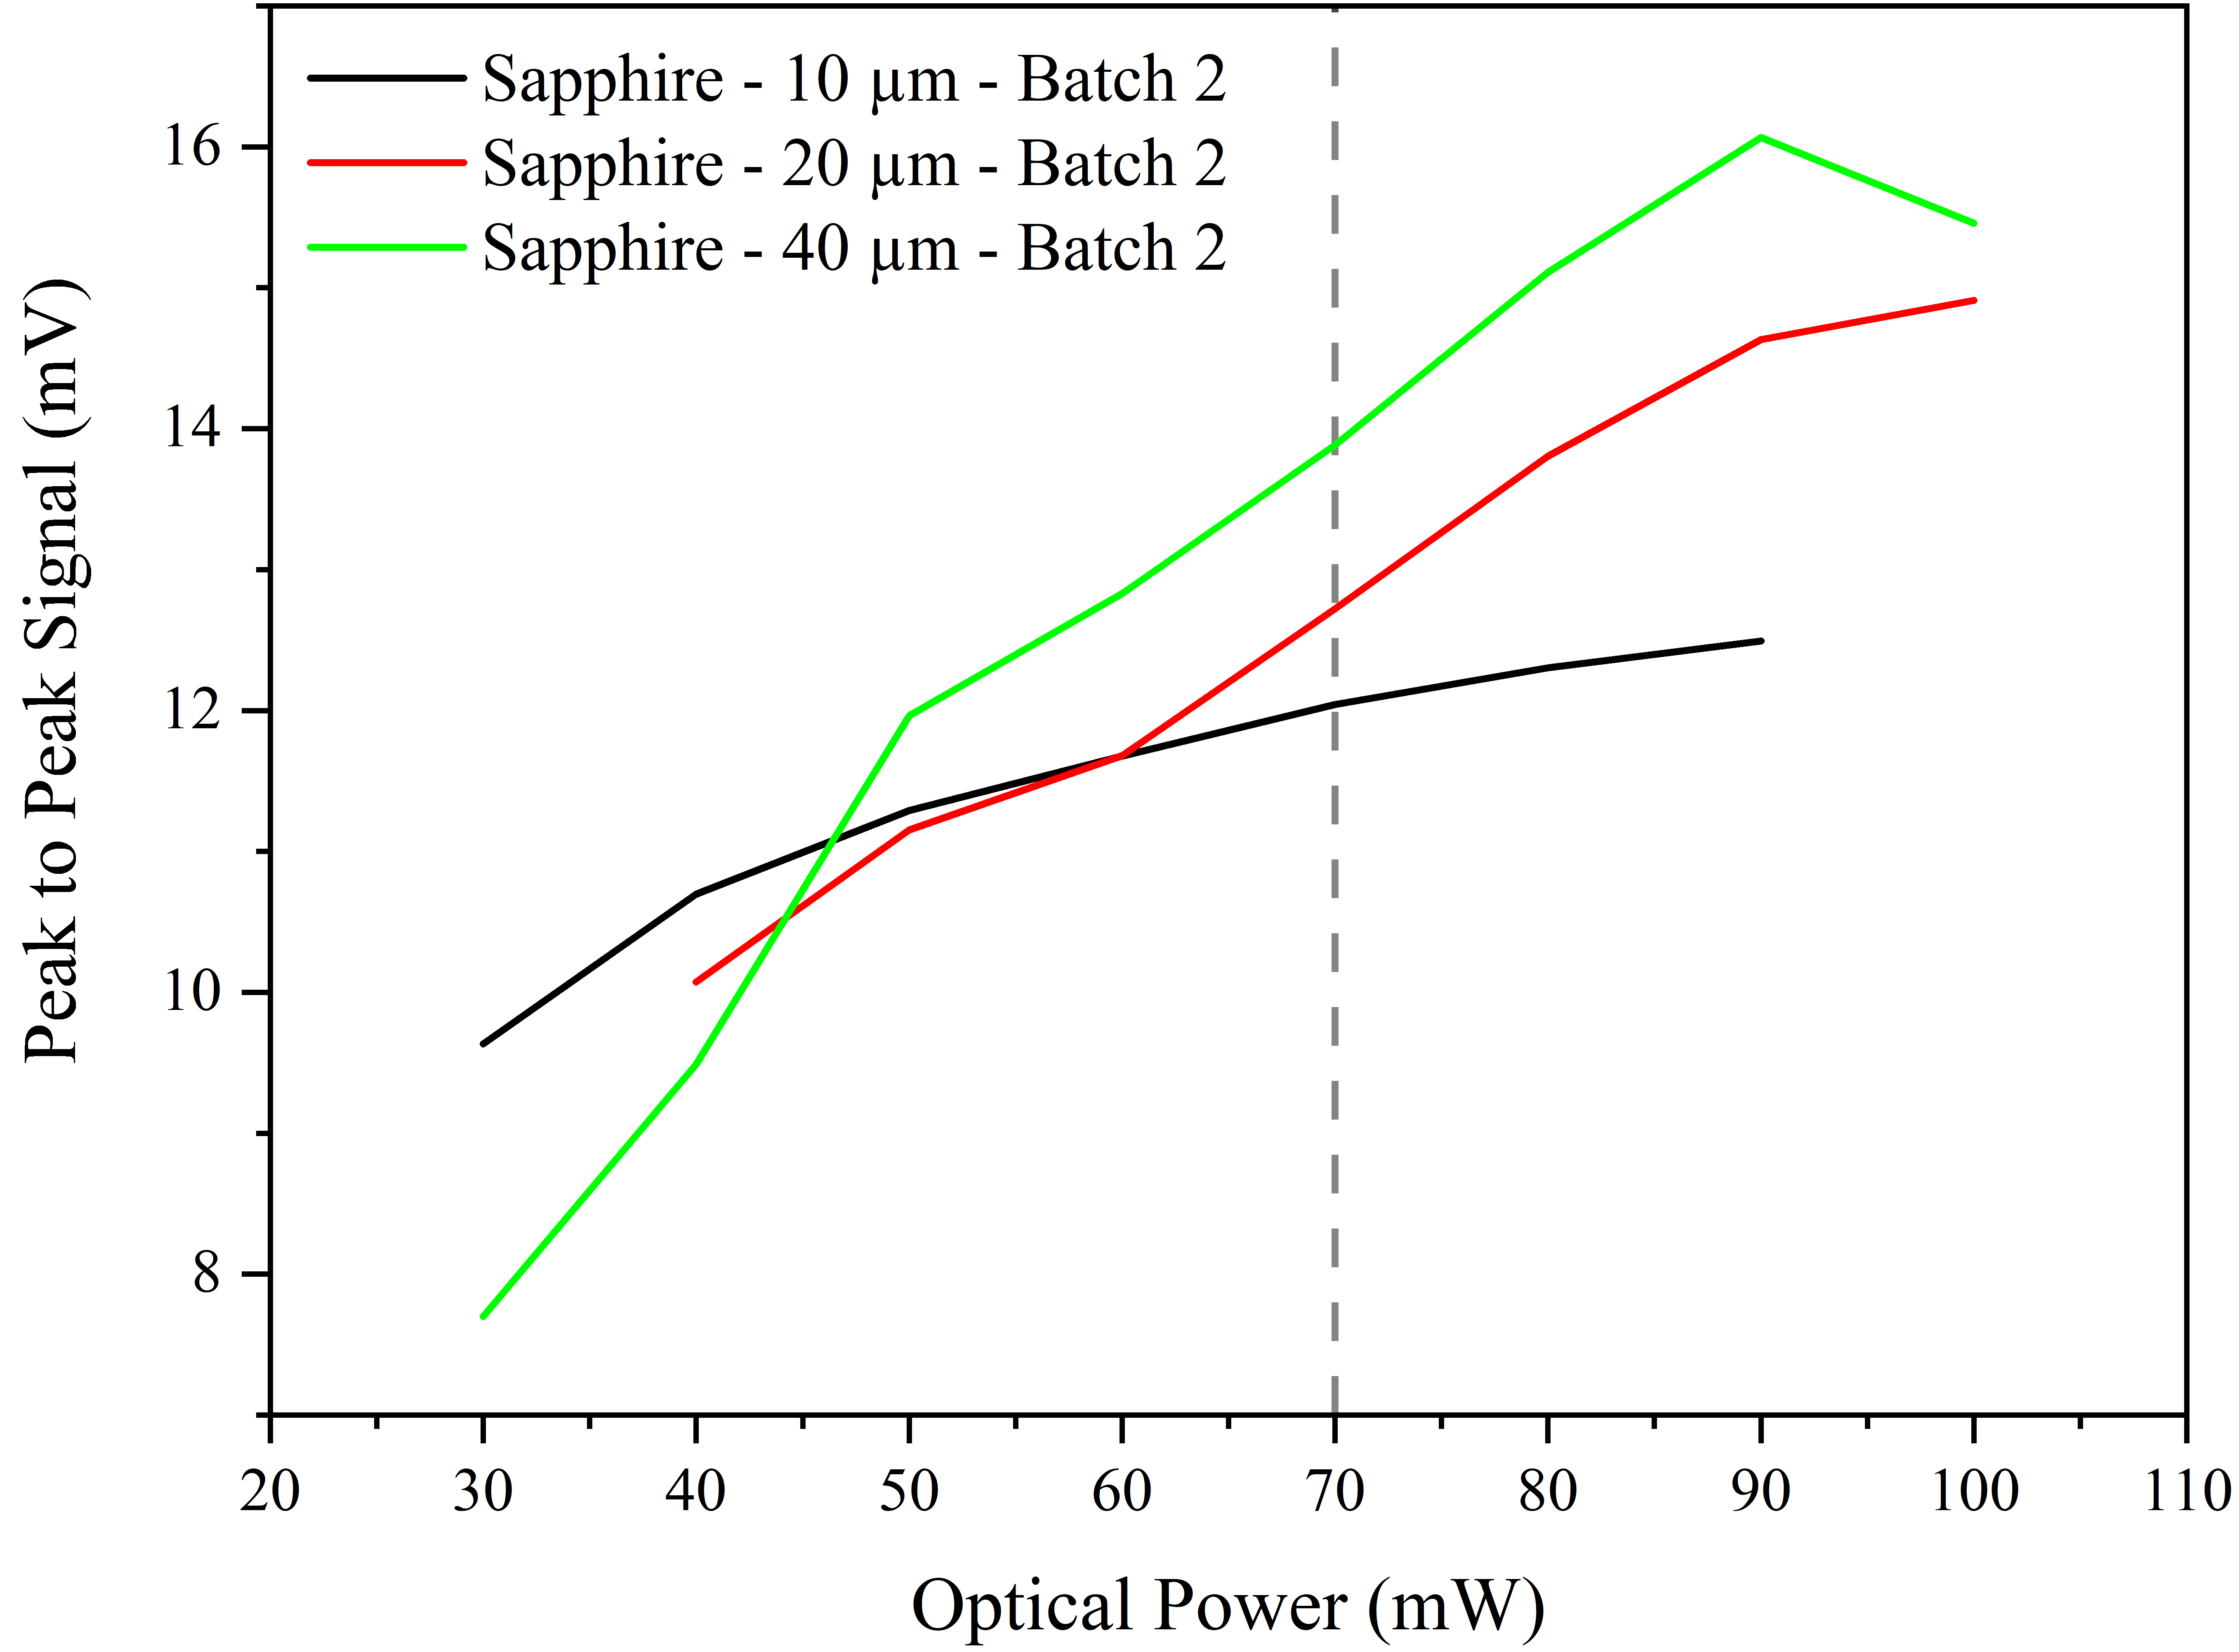
\includegraphics[width=0.6\textwidth]{Figures/Misc/SysDev/OptBatch2Sapph.png}
    \captionsetup{font = footnotesize, justification = centering}
    \caption[The Peak to Peak Signal Values for Sapphire Batch~2]{The peak to peak signal values for Sapphire Batch~2. The trend is reversed from what is expected as the \SI{40}{\micro\metre} device produces the highest output.}
    \label{fig:sapphbatch2}
\end{figure}

It was decided that, for comparison, two devices for each gap size were fabricated using \acrshort{si}\nobreakdash-GaAs as a substrate instead of sapphire. Whilst this is opaque to \SI{800}{\nano\metre} light which only allows front\nobreakdash-side illumination, this is frequently used as a substrate owing to the fewer steps required to fabricate these devices. These sets of devices of 5\nobreakdash--\SI{40}{\micro\metre} will be referred to as GaAs Batch~1 and GaAs Batch~2 respectively. This in particular allows measurements to be performed to determine if the inconsistencies come from problems with the \acrshort{lt}\nobreakdash-GaAs itself, the liftoff and transfer process or the general photolithographic steps when fabricating these small gap devices. The results for these devices are shown individually in \Cref{fig:gaasboth1} and together in \Cref{fig:gaasboth2}. Nearly all these devices seem to follow expected trends well, with all of the 5 and \SI{10}{\micro\metre} devices producing expected relative values. There is some disagreement between batches for the 20 and \SI{40}{\micro\metre} devices but the \SI{40}{\micro\metre} device shows the expected higher saturation tolerance in both batches. As can be seen clearly in \Cref{fig:gaasboth2}, whilst the relative values for each batch are sometimes different, the slopes for each gap size are very similar across batches. 
Owing to the electrical properties of \acrshort{si}\nobreakdash-GaAs, the alignment of these devices was significantly easier than for the sapphire devices. This is because the photocurrent across the device is used for initial alignment and \acrshort{si}\nobreakdash-GaAs generated significantly more photocurrent for a given applied bias and incident optical power, which is a proxy for the alignment of the beam spot across the devices gap. This is a result of the much higher conductivity of \acrshort{si}\nobreakdash-GaAs which results in parasitic photocurrent being generated within the \acrshort{si}\nobreakdash-GaAs substrate.

\begin{figure}[ht!]%t
\centering
\begin{subfigure}{1\textwidth}
    \centering
    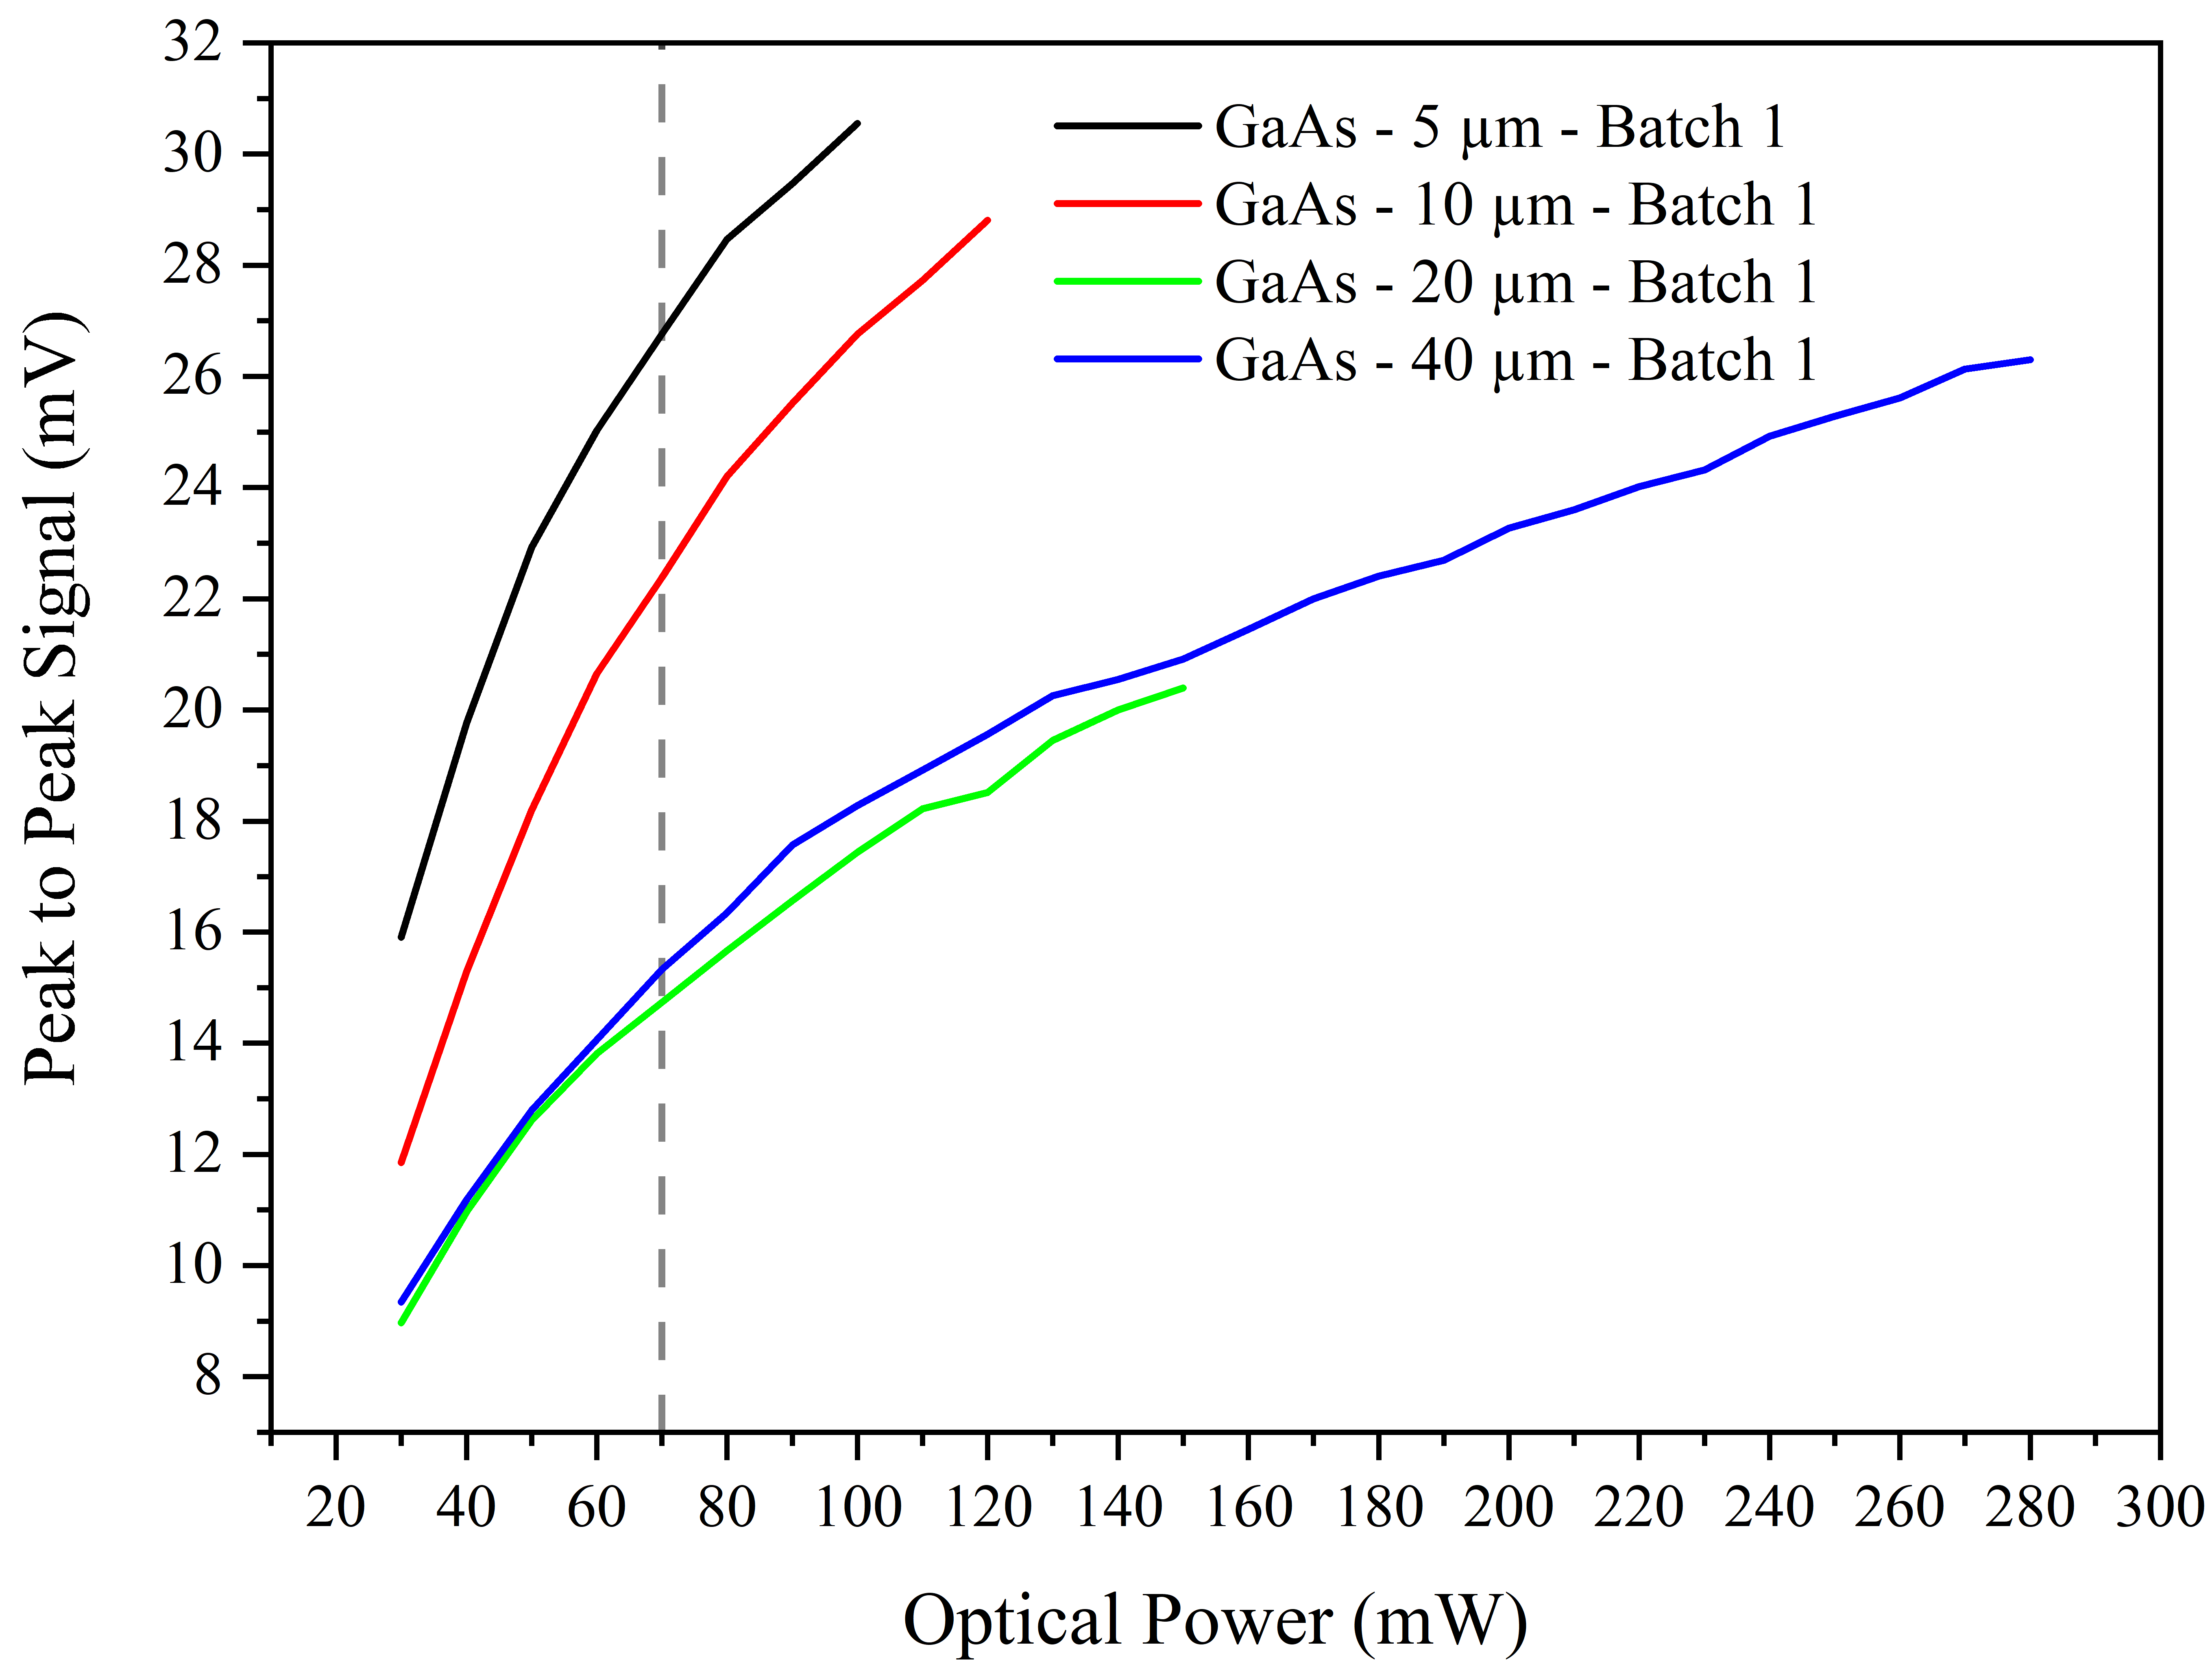
\includegraphics[scale=0.4]{Figures/Misc/SysDev/OptGaAsBatch1G.png}
    \caption{The peak to peak signal values for GaAs Batch~1.}
    \label{fig:gaasbatch1}
\end{subfigure}
\begin{subfigure}{1\textwidth}
    \centering
    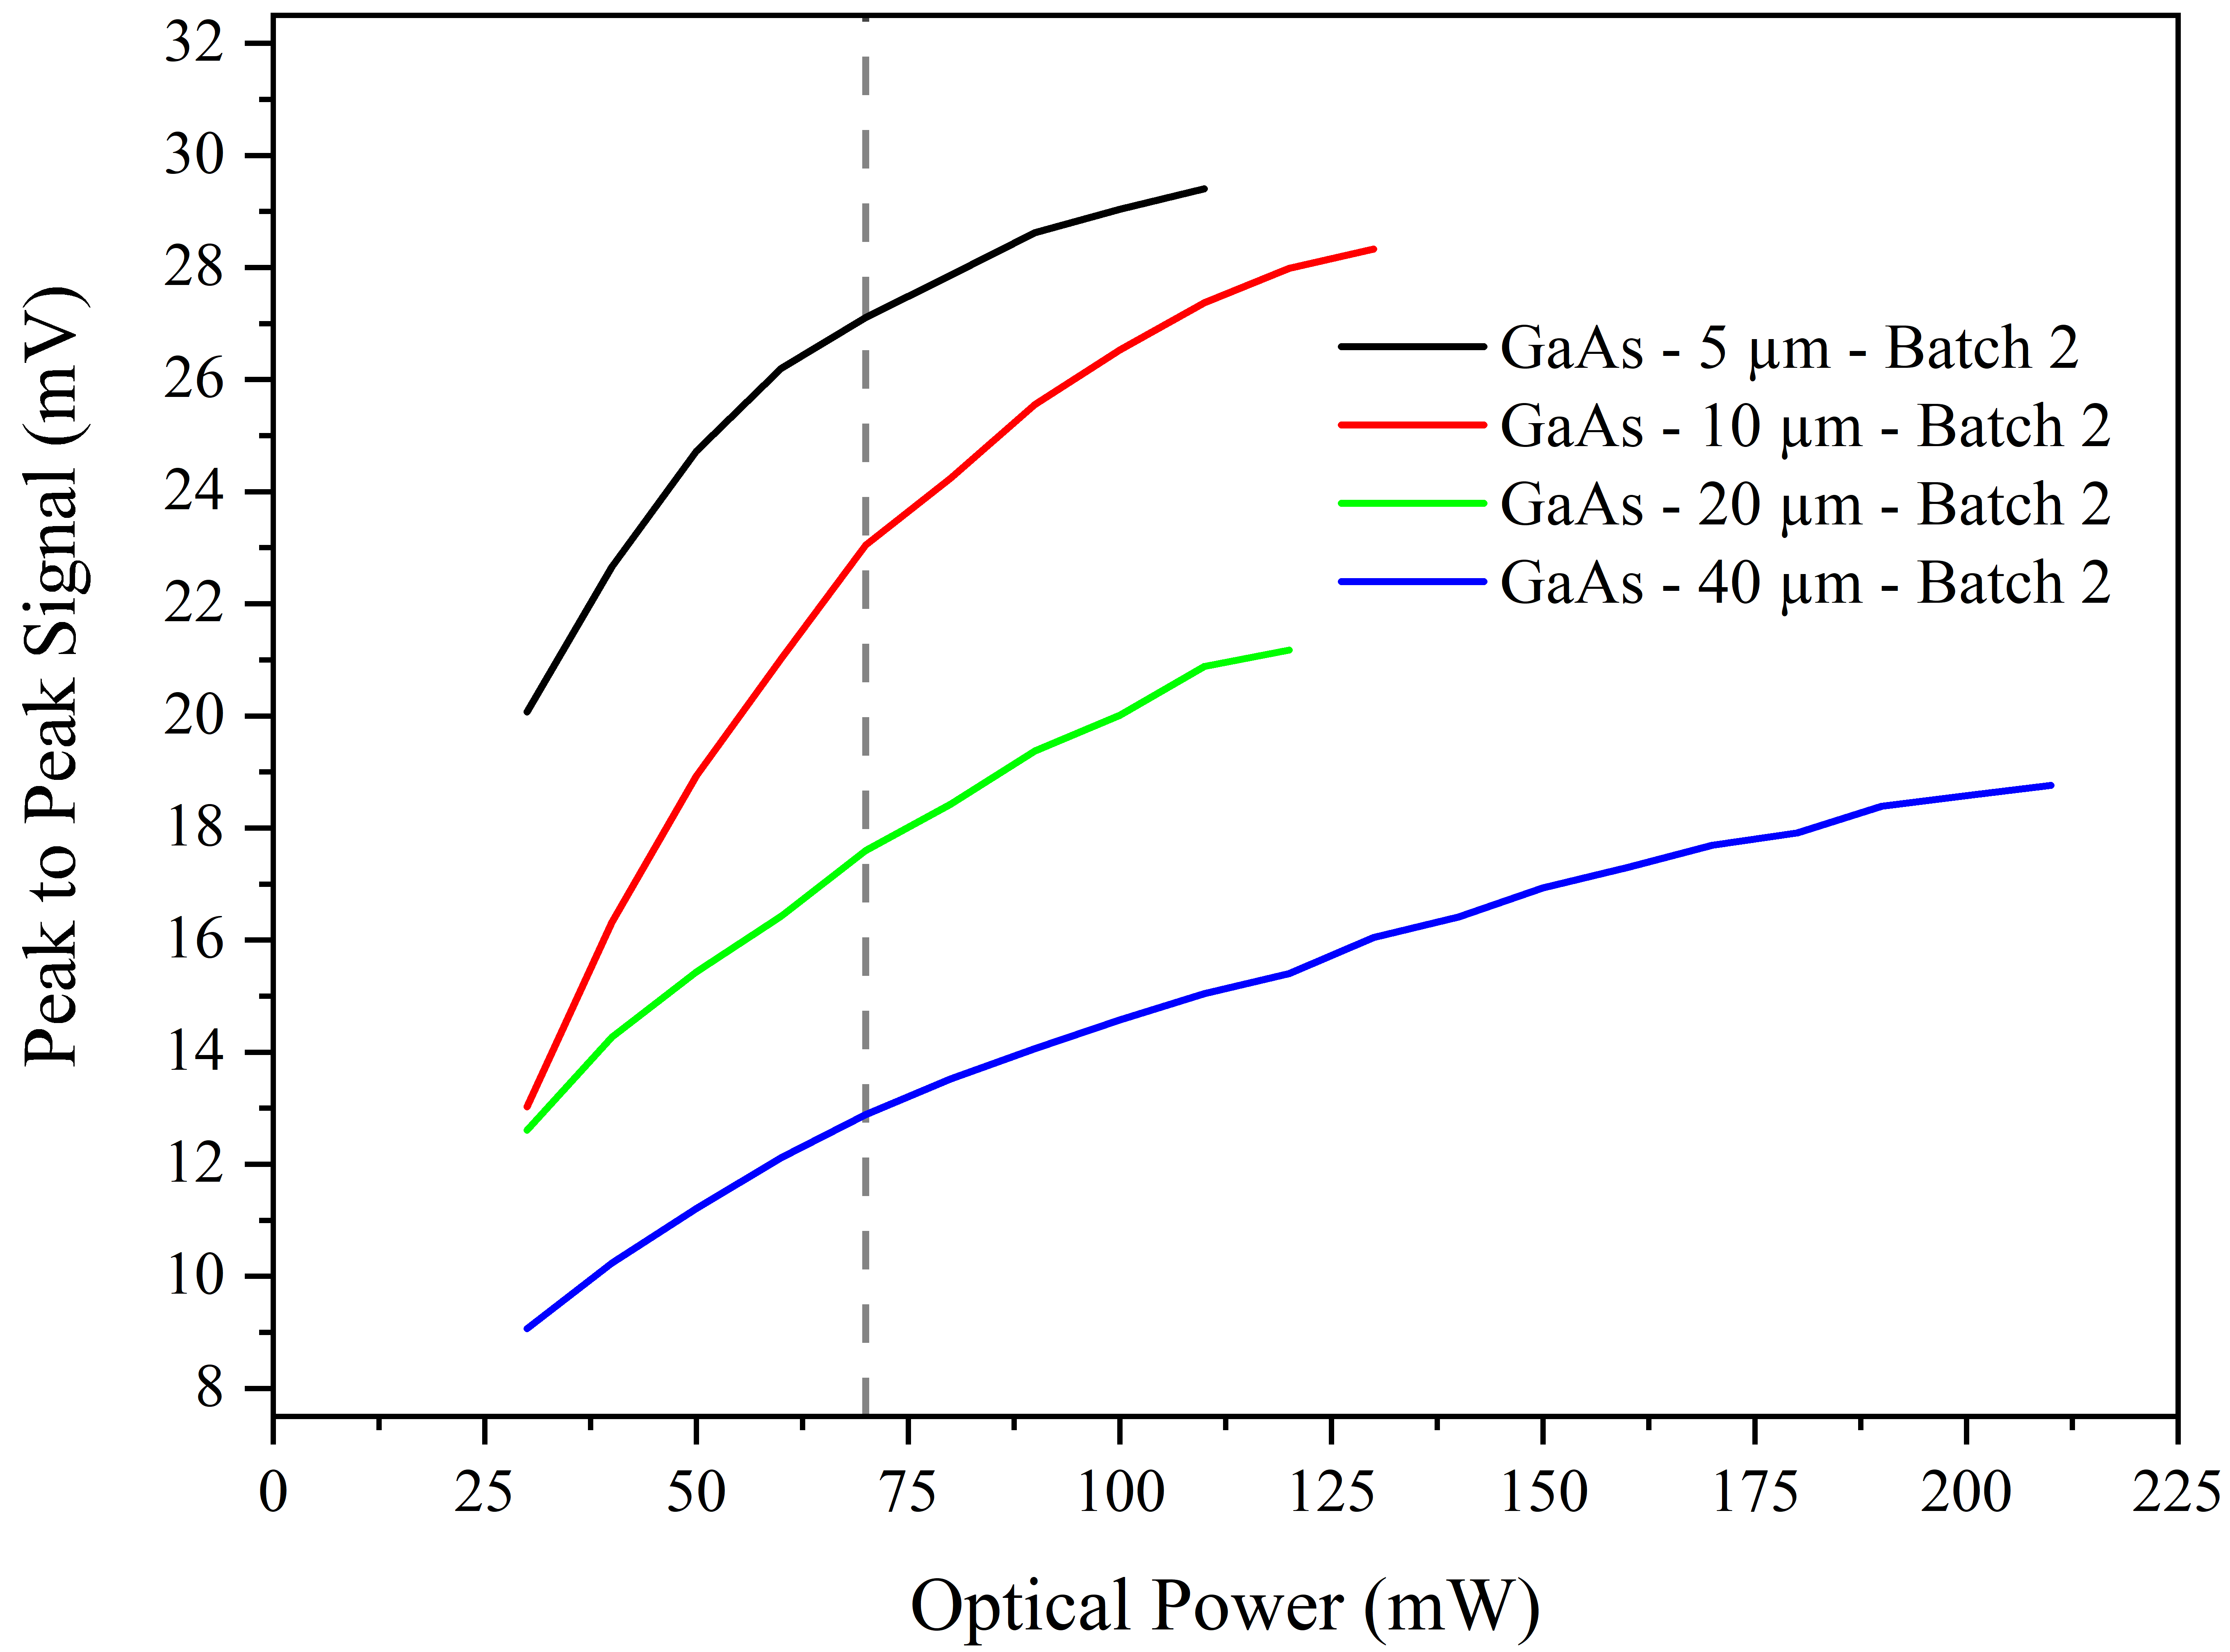
\includegraphics[scale=0.4]{Figures/Misc/SysDev/OptGaAsBatch2G.png}
    \caption{The peak to peak signal values for GaAs Batch~2.}
    \label{fig:gaasbatch2}
\end{subfigure}
\captionsetup{font = footnotesize, justification = centering}
\caption[The Peak to Peak Signal Values for both GaAs Batches - Seperate]{The peak to peak signal values for both GaAs batches. These generally follow expected trends with the exception of the \SI{20}{\micro\metre} device in GaAs Batch~2 under\nobreakdash-performing. The improved output of these devices is likely down to their increased photocurrent which improves alignment.}
\label{fig:gaasboth1}
\end{figure}

\begin{figure}[h]
    \centering
    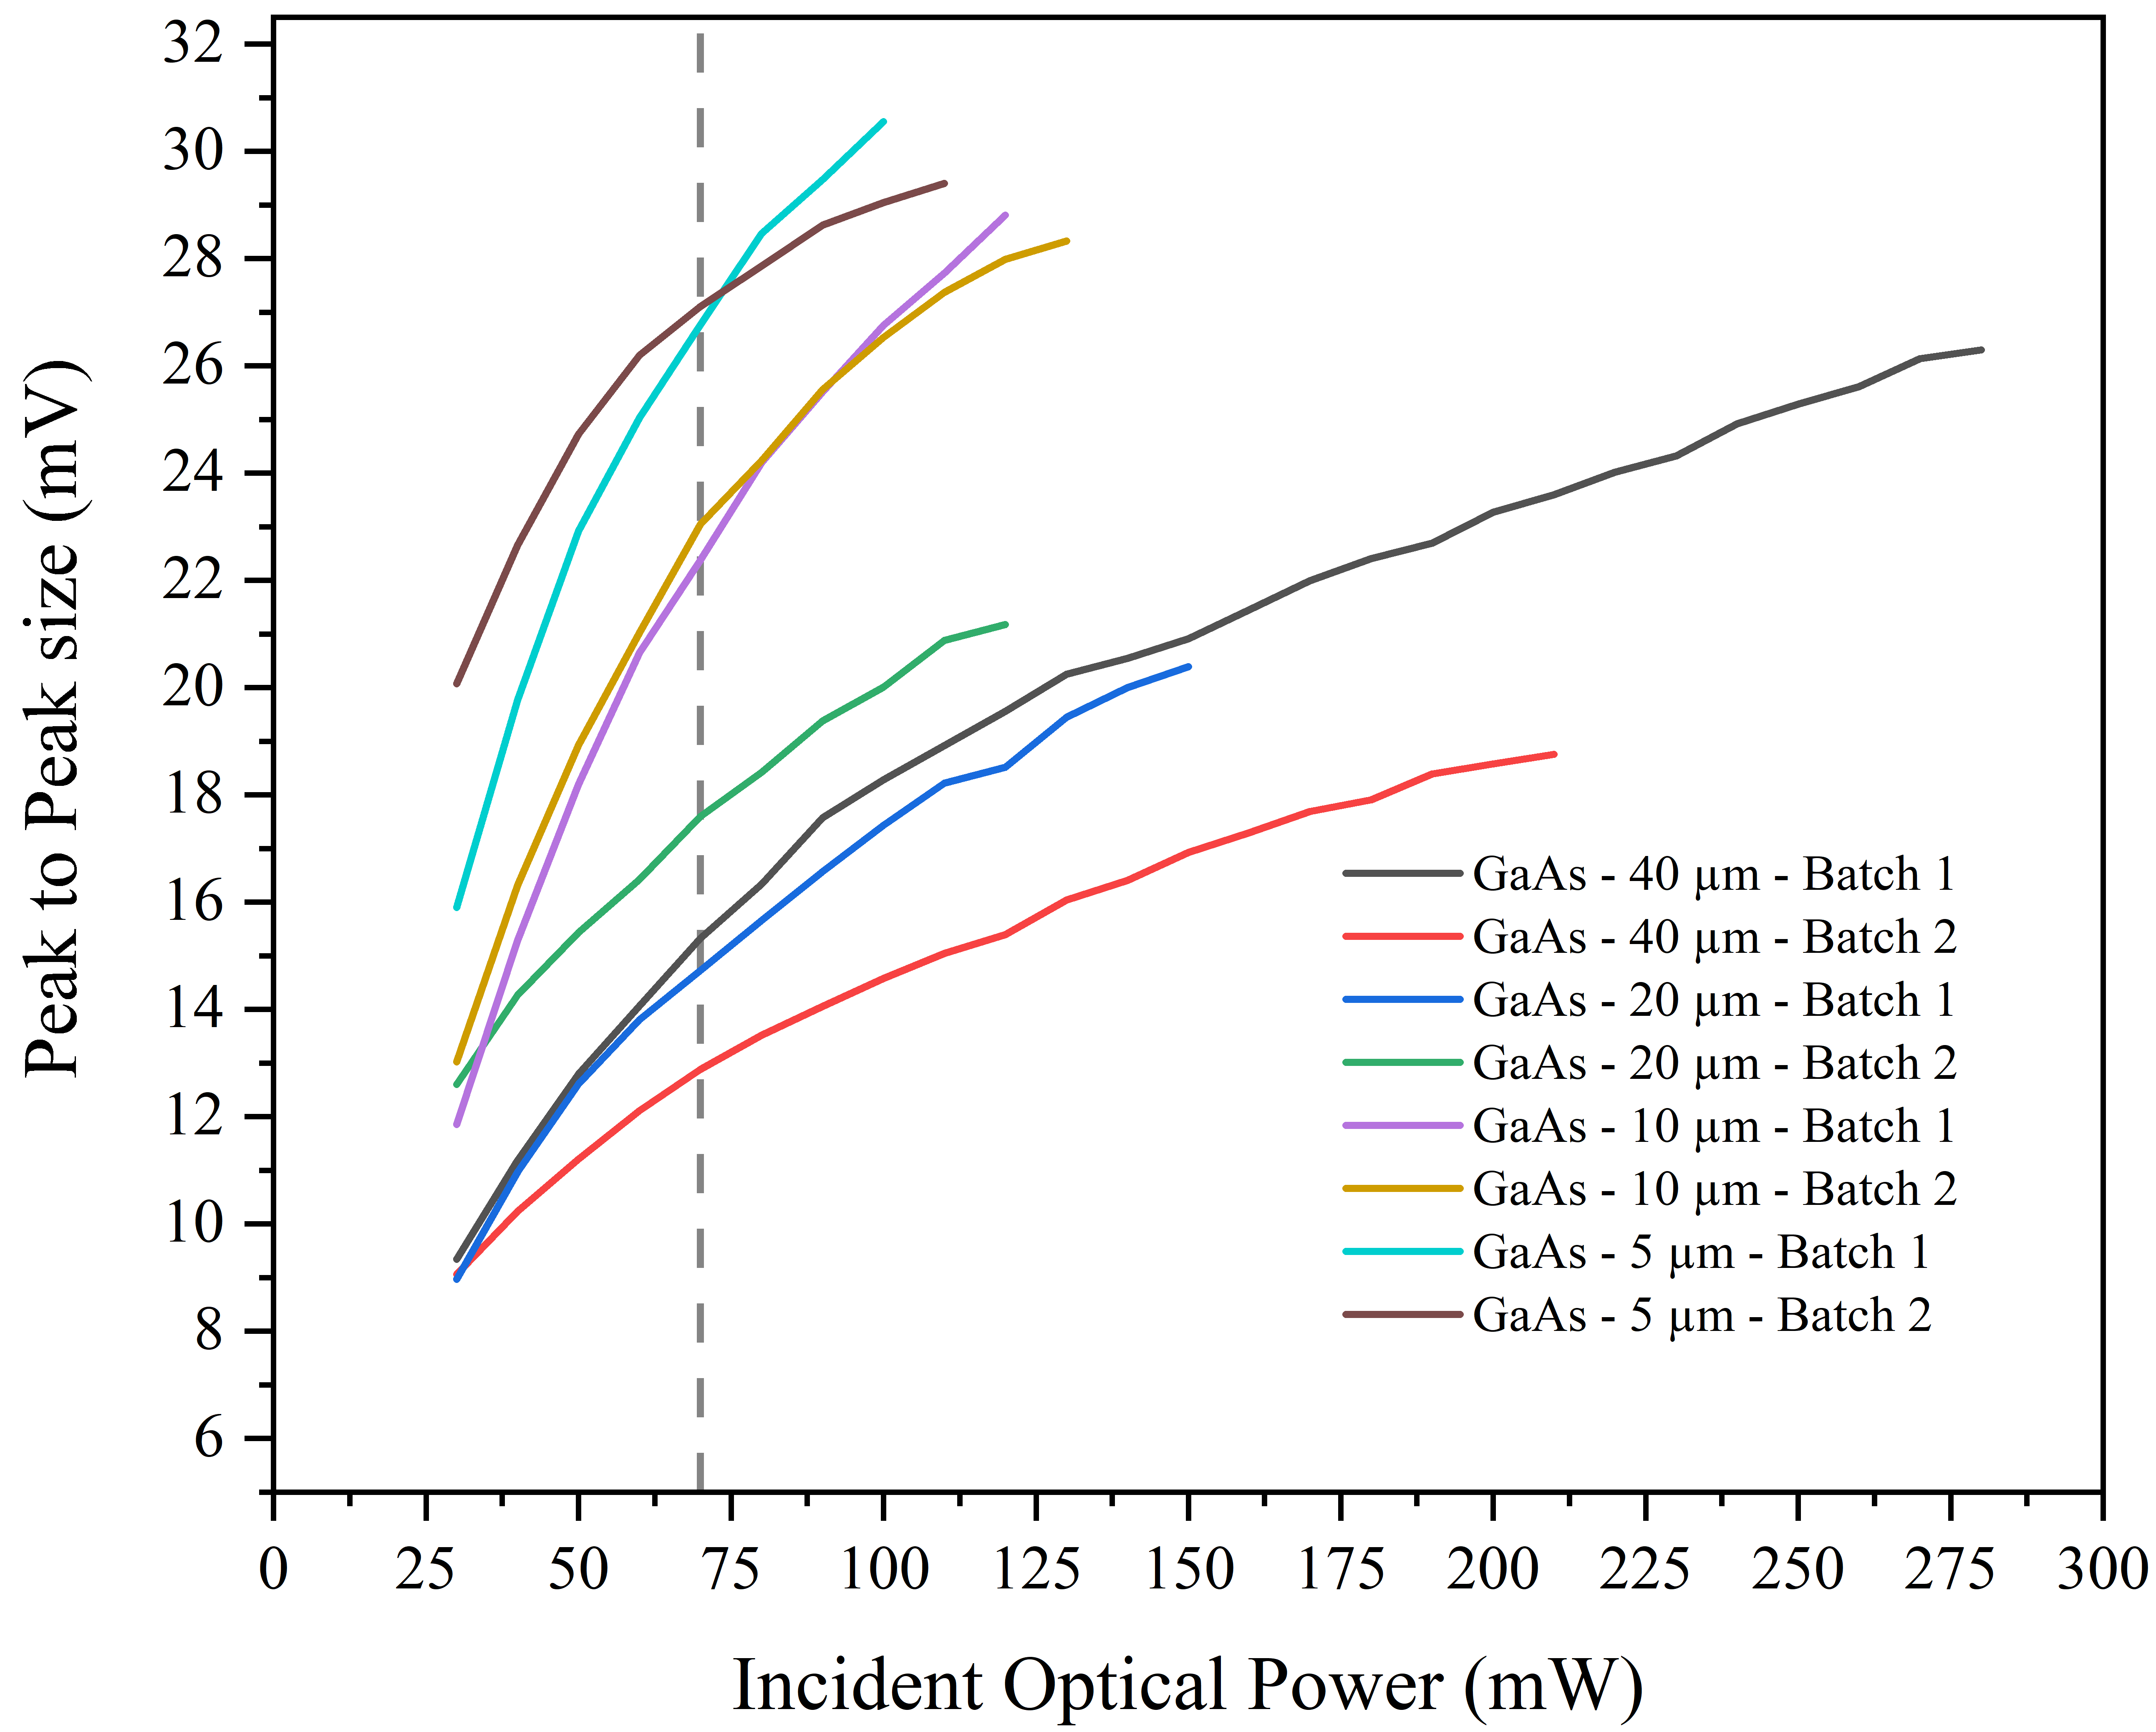
\includegraphics[width=0.7\textwidth]{Figures/Misc/SysDev/OptGaAsBothG.png}
    \captionsetup{font = footnotesize, justification = centering}
    \caption[The Peak to Peak Signal Values for both GaAs Batches - Combined]{The peak to peak signal values for both GaAs batches. It can be seen that the saturation behaviour across batches is consistent.}
    \label{fig:gaasboth2}
\end{figure}

A final batch of emitters were fabricated using a sapphire substrate and tested as described above. These are shown in \Cref{fig:sapphbatch3} and will be referred to as Sapphire Batch~3. Owing to difficulties during alignment, both the 5 and \SI{10}{\micro\metre} devices were destroyed before data could be obtained. The remaining devices show the expected signal size trends but the \SI{40}{\micro\metre} device begins to saturate before the \SI{20}{\micro\metre} device which does not agree with previous results. This, again, can likely be accounted for with alignment issues and fabrication defects.

\begin{figure}[h!t]%t
    \centering
    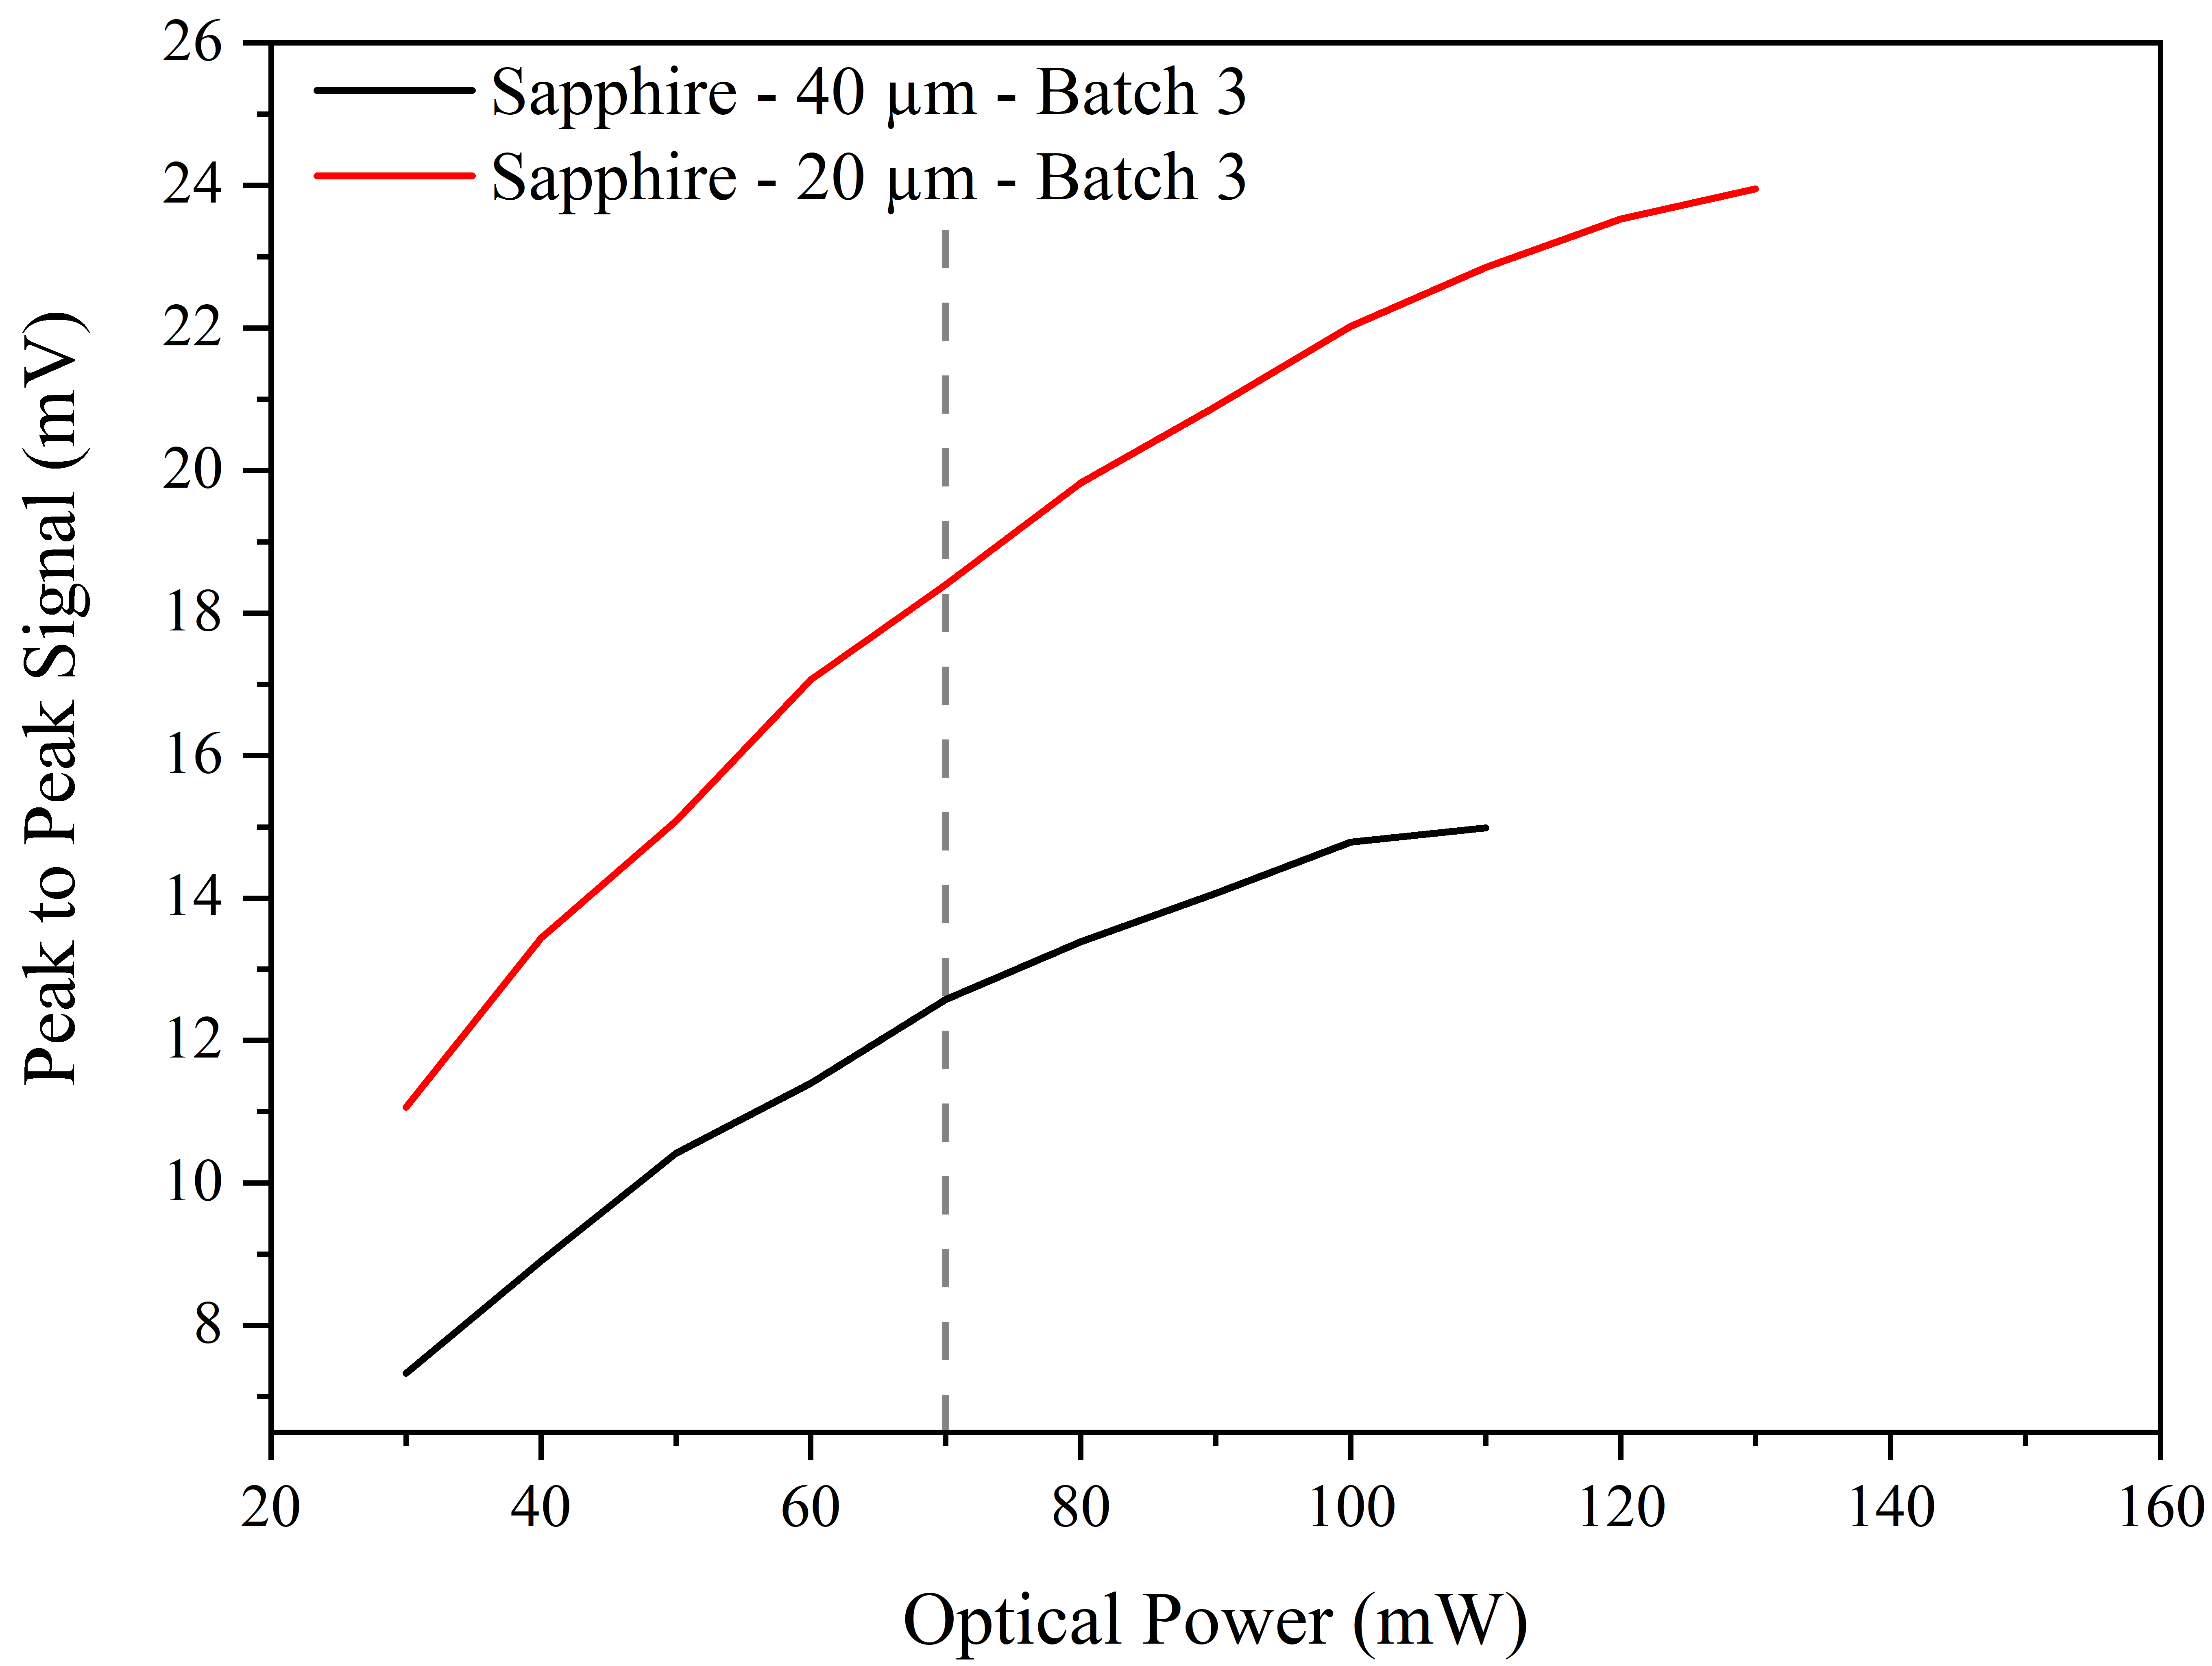
\includegraphics[width=0.6\textwidth]{Figures/Misc/SysDev/OptSapphBatch3.png}
    \captionsetup{font = footnotesize, justification = centering}
    \caption[The Peak to Peak Signal Values for Sapphire Batch~3]{The peak to peak signal values for Sapphire Batch~3. Whilst it is expected that the \SI{20}{\micro\metre} would produce a higher output, it was expected to saturate earlier which has not happened.}
    \label{fig:sapphbatch3}
\end{figure}

The results for all the devices with gap size of \SI{10}{\micro\metre} are shown in \Cref{fig:10micron}. There seems to be some discrepancy within the Sapphire batches which is likely owing to difficulties in aligning the Sapphire devices and defects introduced during their fabrication and the GaAs devices outperform the sapphire devices. The results of all the devices with gap size of \SI{20}{\micro\metre} are shown in \Cref{fig:20micron}, where the sapphire devices show quite large disagreement in both output and saturation behavior but the GaAs devices are reasonably consistent. This could also be caused by issues with the Au electrodes whereby they do not bind uniformly across the device owing to discrepancies in the photoresist coverage. Finally the results for all the devices with gap size of \SI{40}{\micro\metre} are shown in \Cref{fig:s40micron}. The saturation behavior for these devices is radically different than expected, with the sapphire devices saturating well before the GaAs devices. A \SI{20}{\micro\metre} device on sapphire at \SI{20}{V} has a dark current of approximately \SI{0.0018}{\micro\ampere} whilst a \SI{20}{\micro\metre} device on GaAs at \SI{20}{V} has a dark current of approximately \SI{0.0362}{\micro\ampere}. This is almost a 200\% increase in the level of dark current between substrates. However, this only makes a significant difference at high applied biases \DIFdelbegin \DIFdel{~}\DIFdelend \cite{Bacon2016}. The out\nobreakdash-performance of the GaAs devices when compared to the Sapphire devices can possibly be attributed to low applied fields and incident optical powers involved.

\begin{figure}[h!]
    \centering
    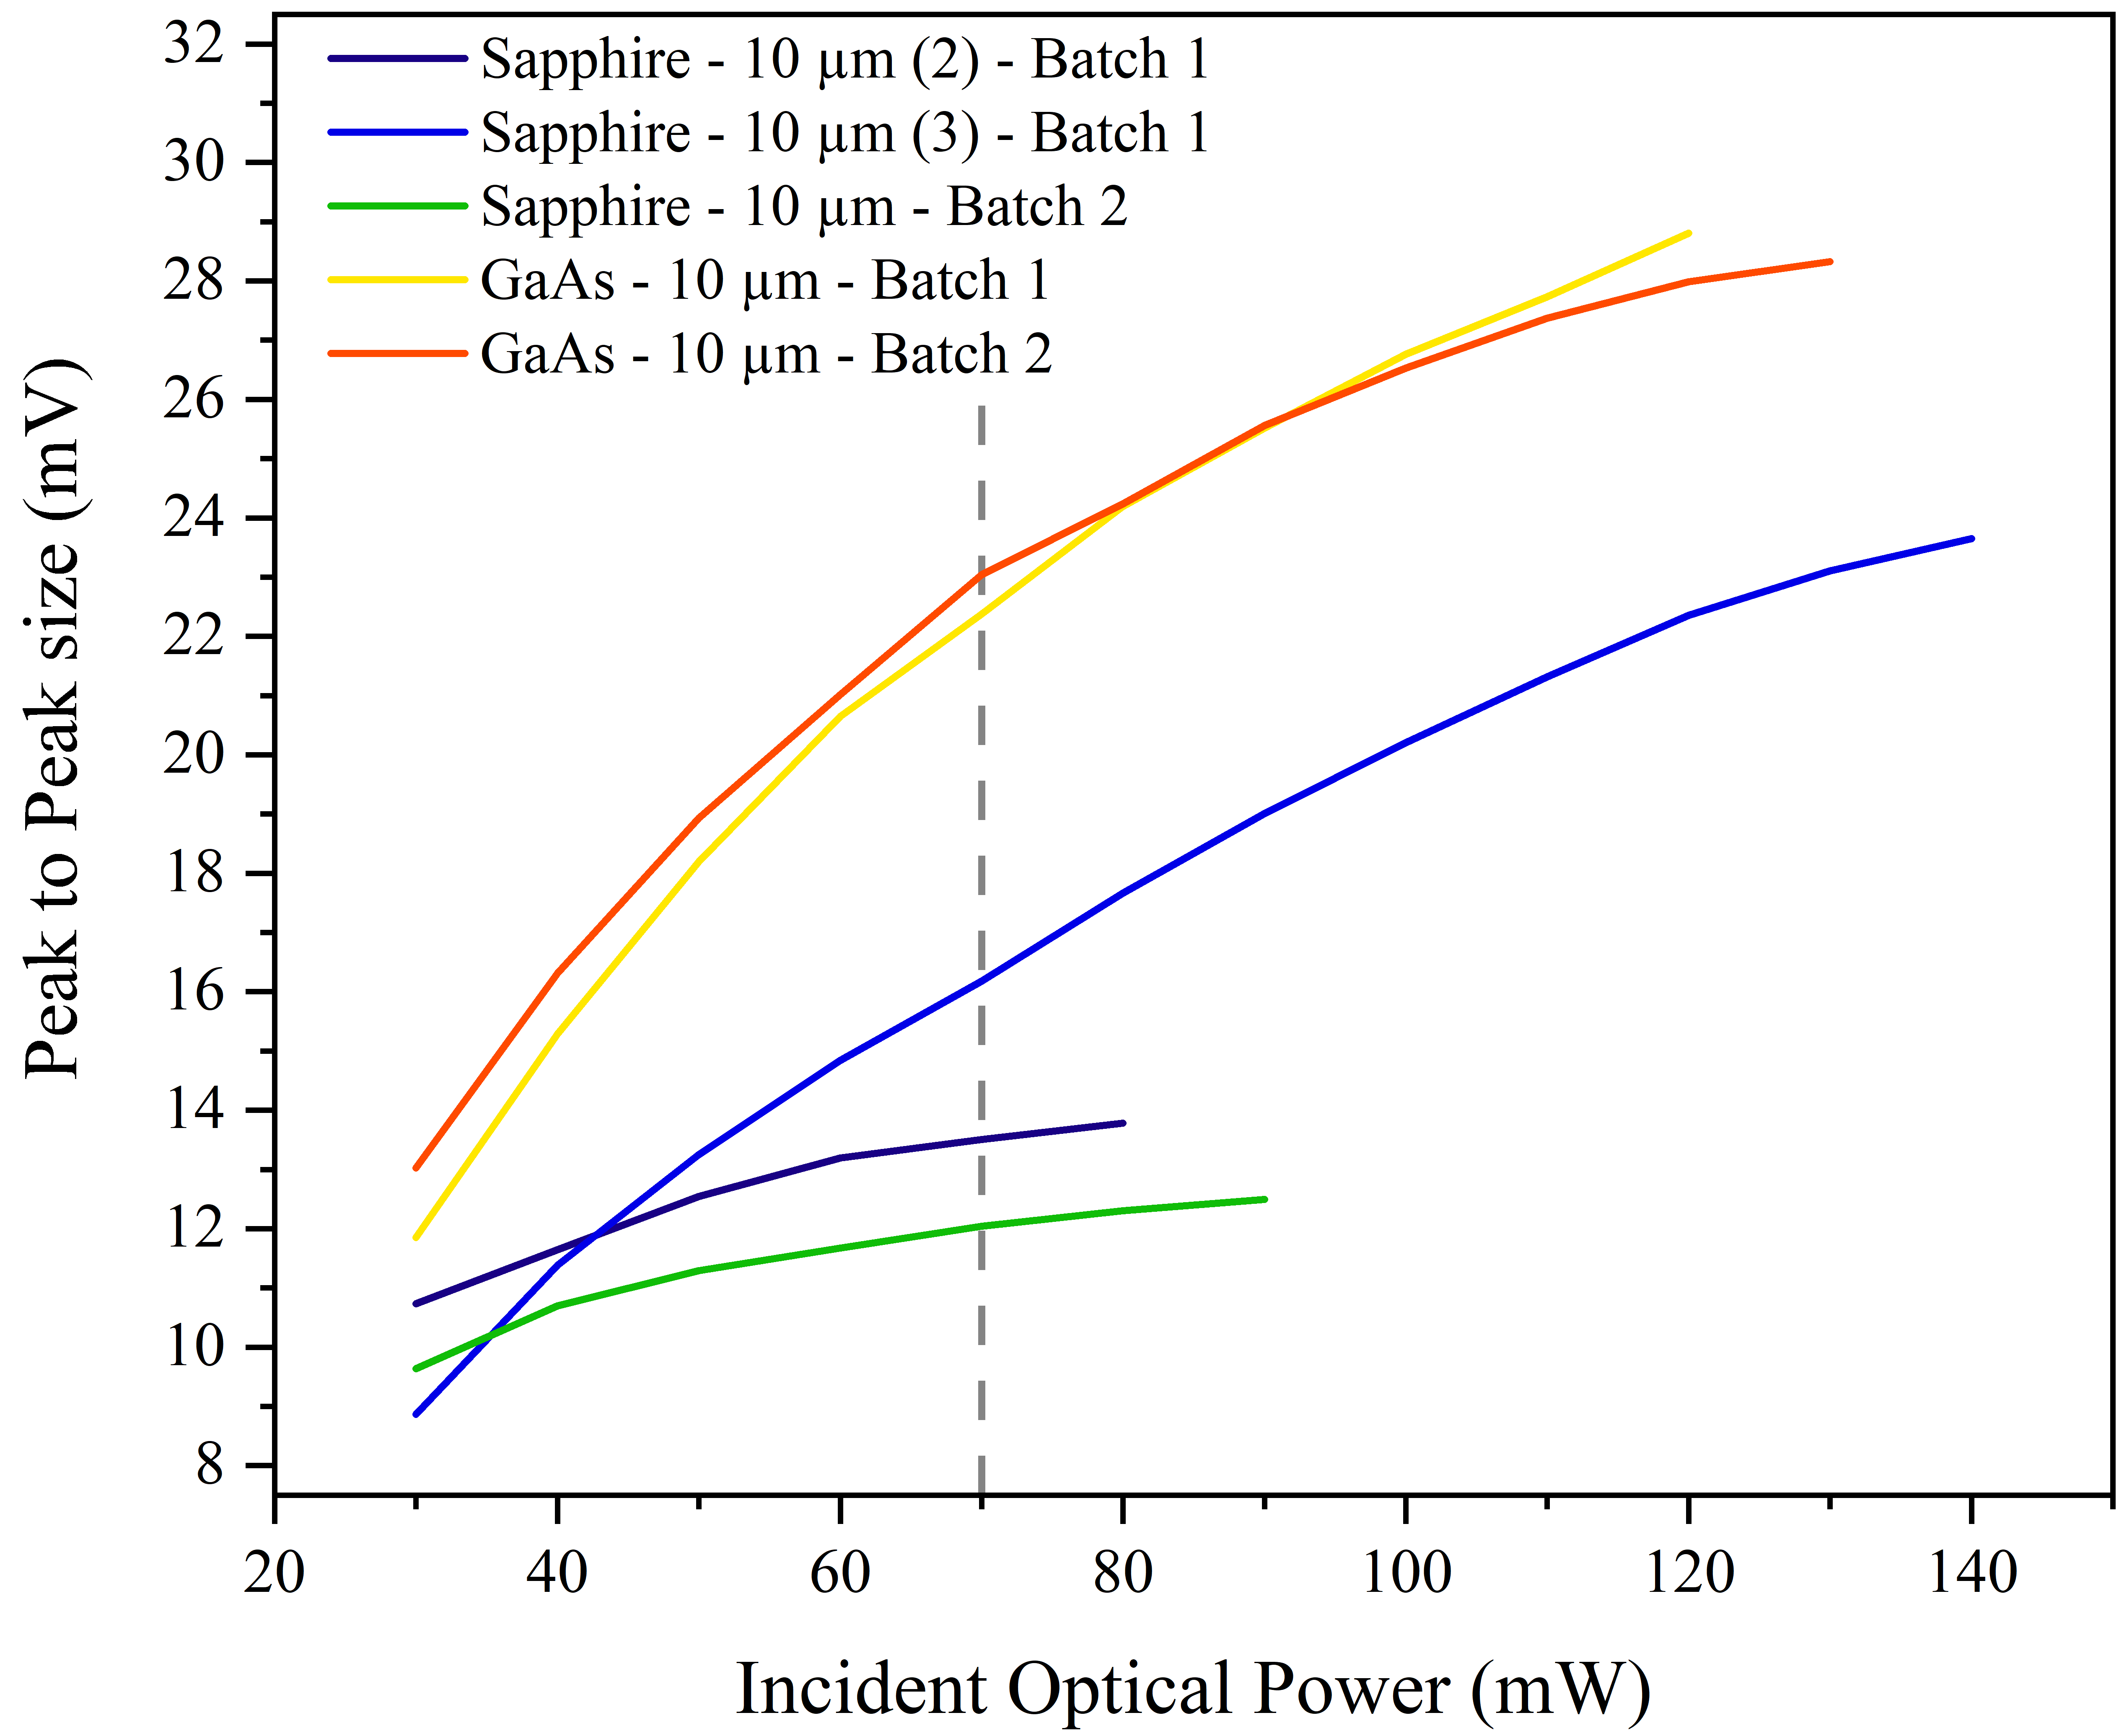
\includegraphics[width=0.6\textwidth]{Figures/Misc/SysDev/Opt10micronG.png}
    \captionsetup{font = footnotesize, justification = centering}
    \caption[The Peak to Peak Signal Values for all Devices with \SI{10}{\micro\metre} Gap]{The peak to peak signal values for all devices with a gap size of \SI{10}{\micro\metre}. There is disagreement between the sapphire batches but saturation behaviour and output are consistent within batches.}
    \label{fig:10micron}
\end{figure}

\begin{figure}[h!]
    \centering
    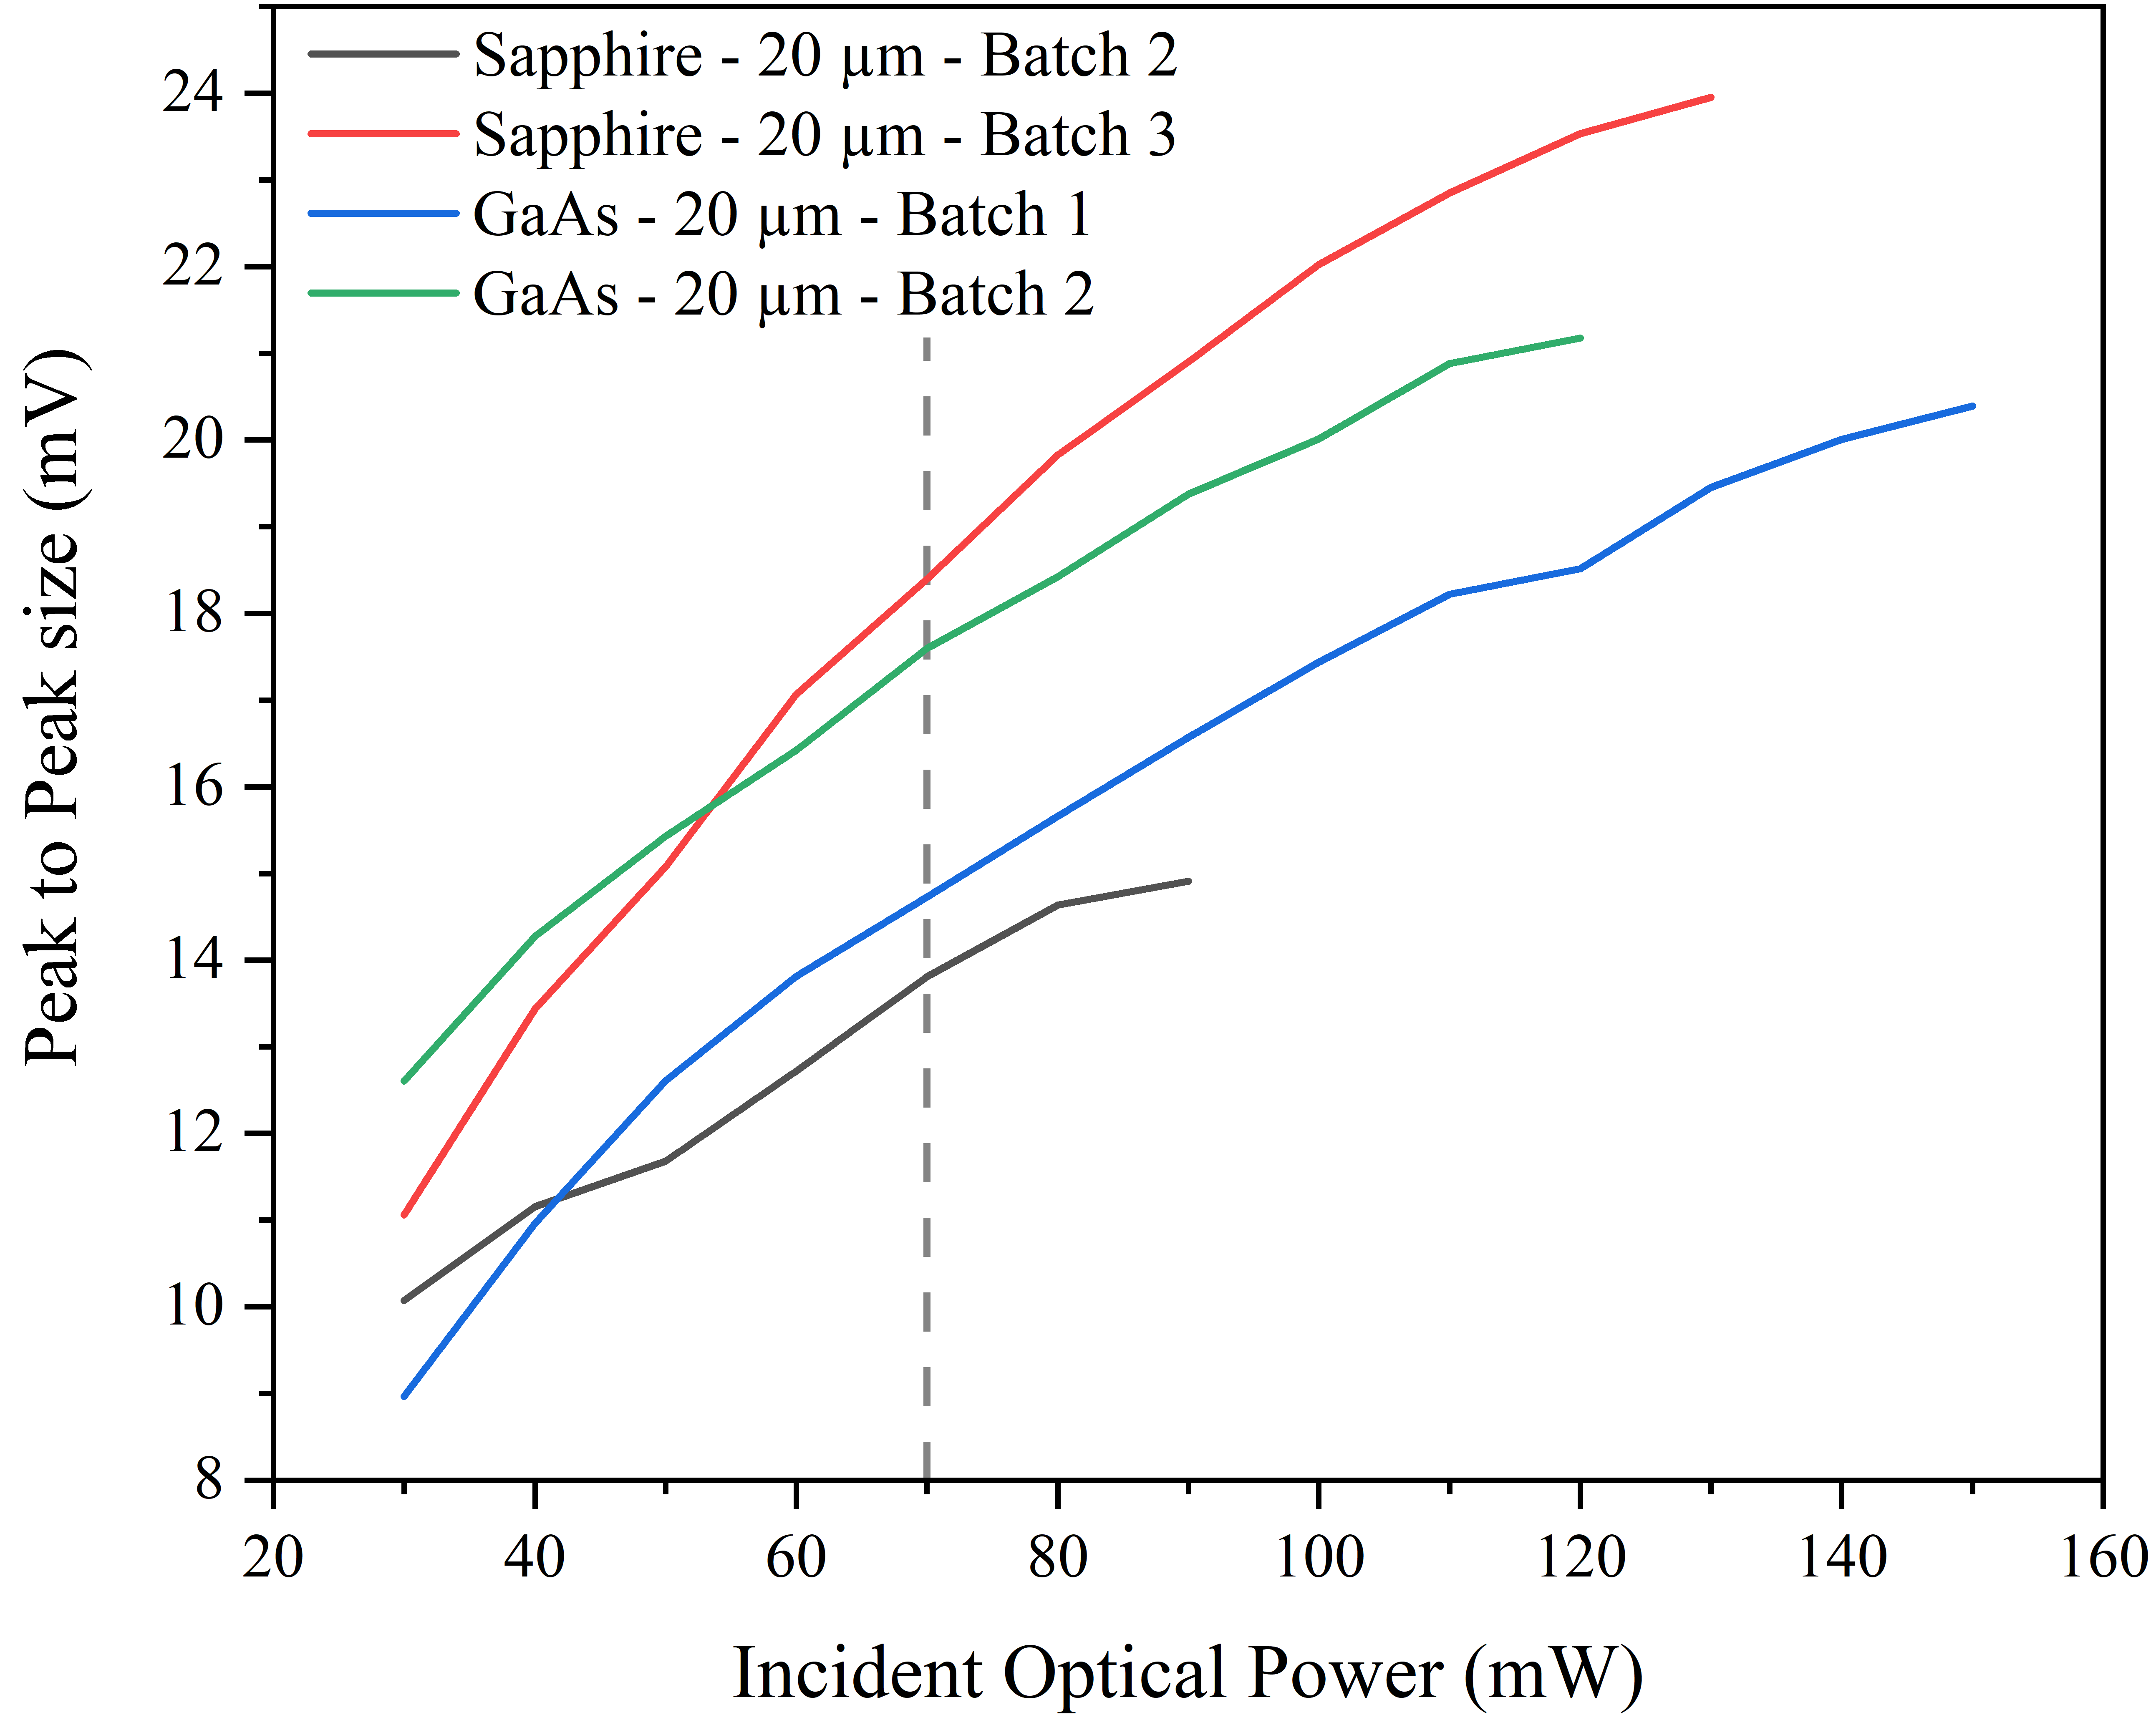
\includegraphics[width=0.6\textwidth]{Figures/Misc/SysDev/Opt20micronG.png}
    \captionsetup{font = footnotesize, justification = centering}
    \caption[The Peak to Peak Signal Values for all Devices with \SI{20}{\micro\metre} Gap]{The peak to peak signal values for all devices with a gap size of \SI{20}{\micro\metre}. The sapphire devices show significant disagreement.}
    \label{fig:20micron}
\end{figure}

\begin{figure}[h!]
    \centering
    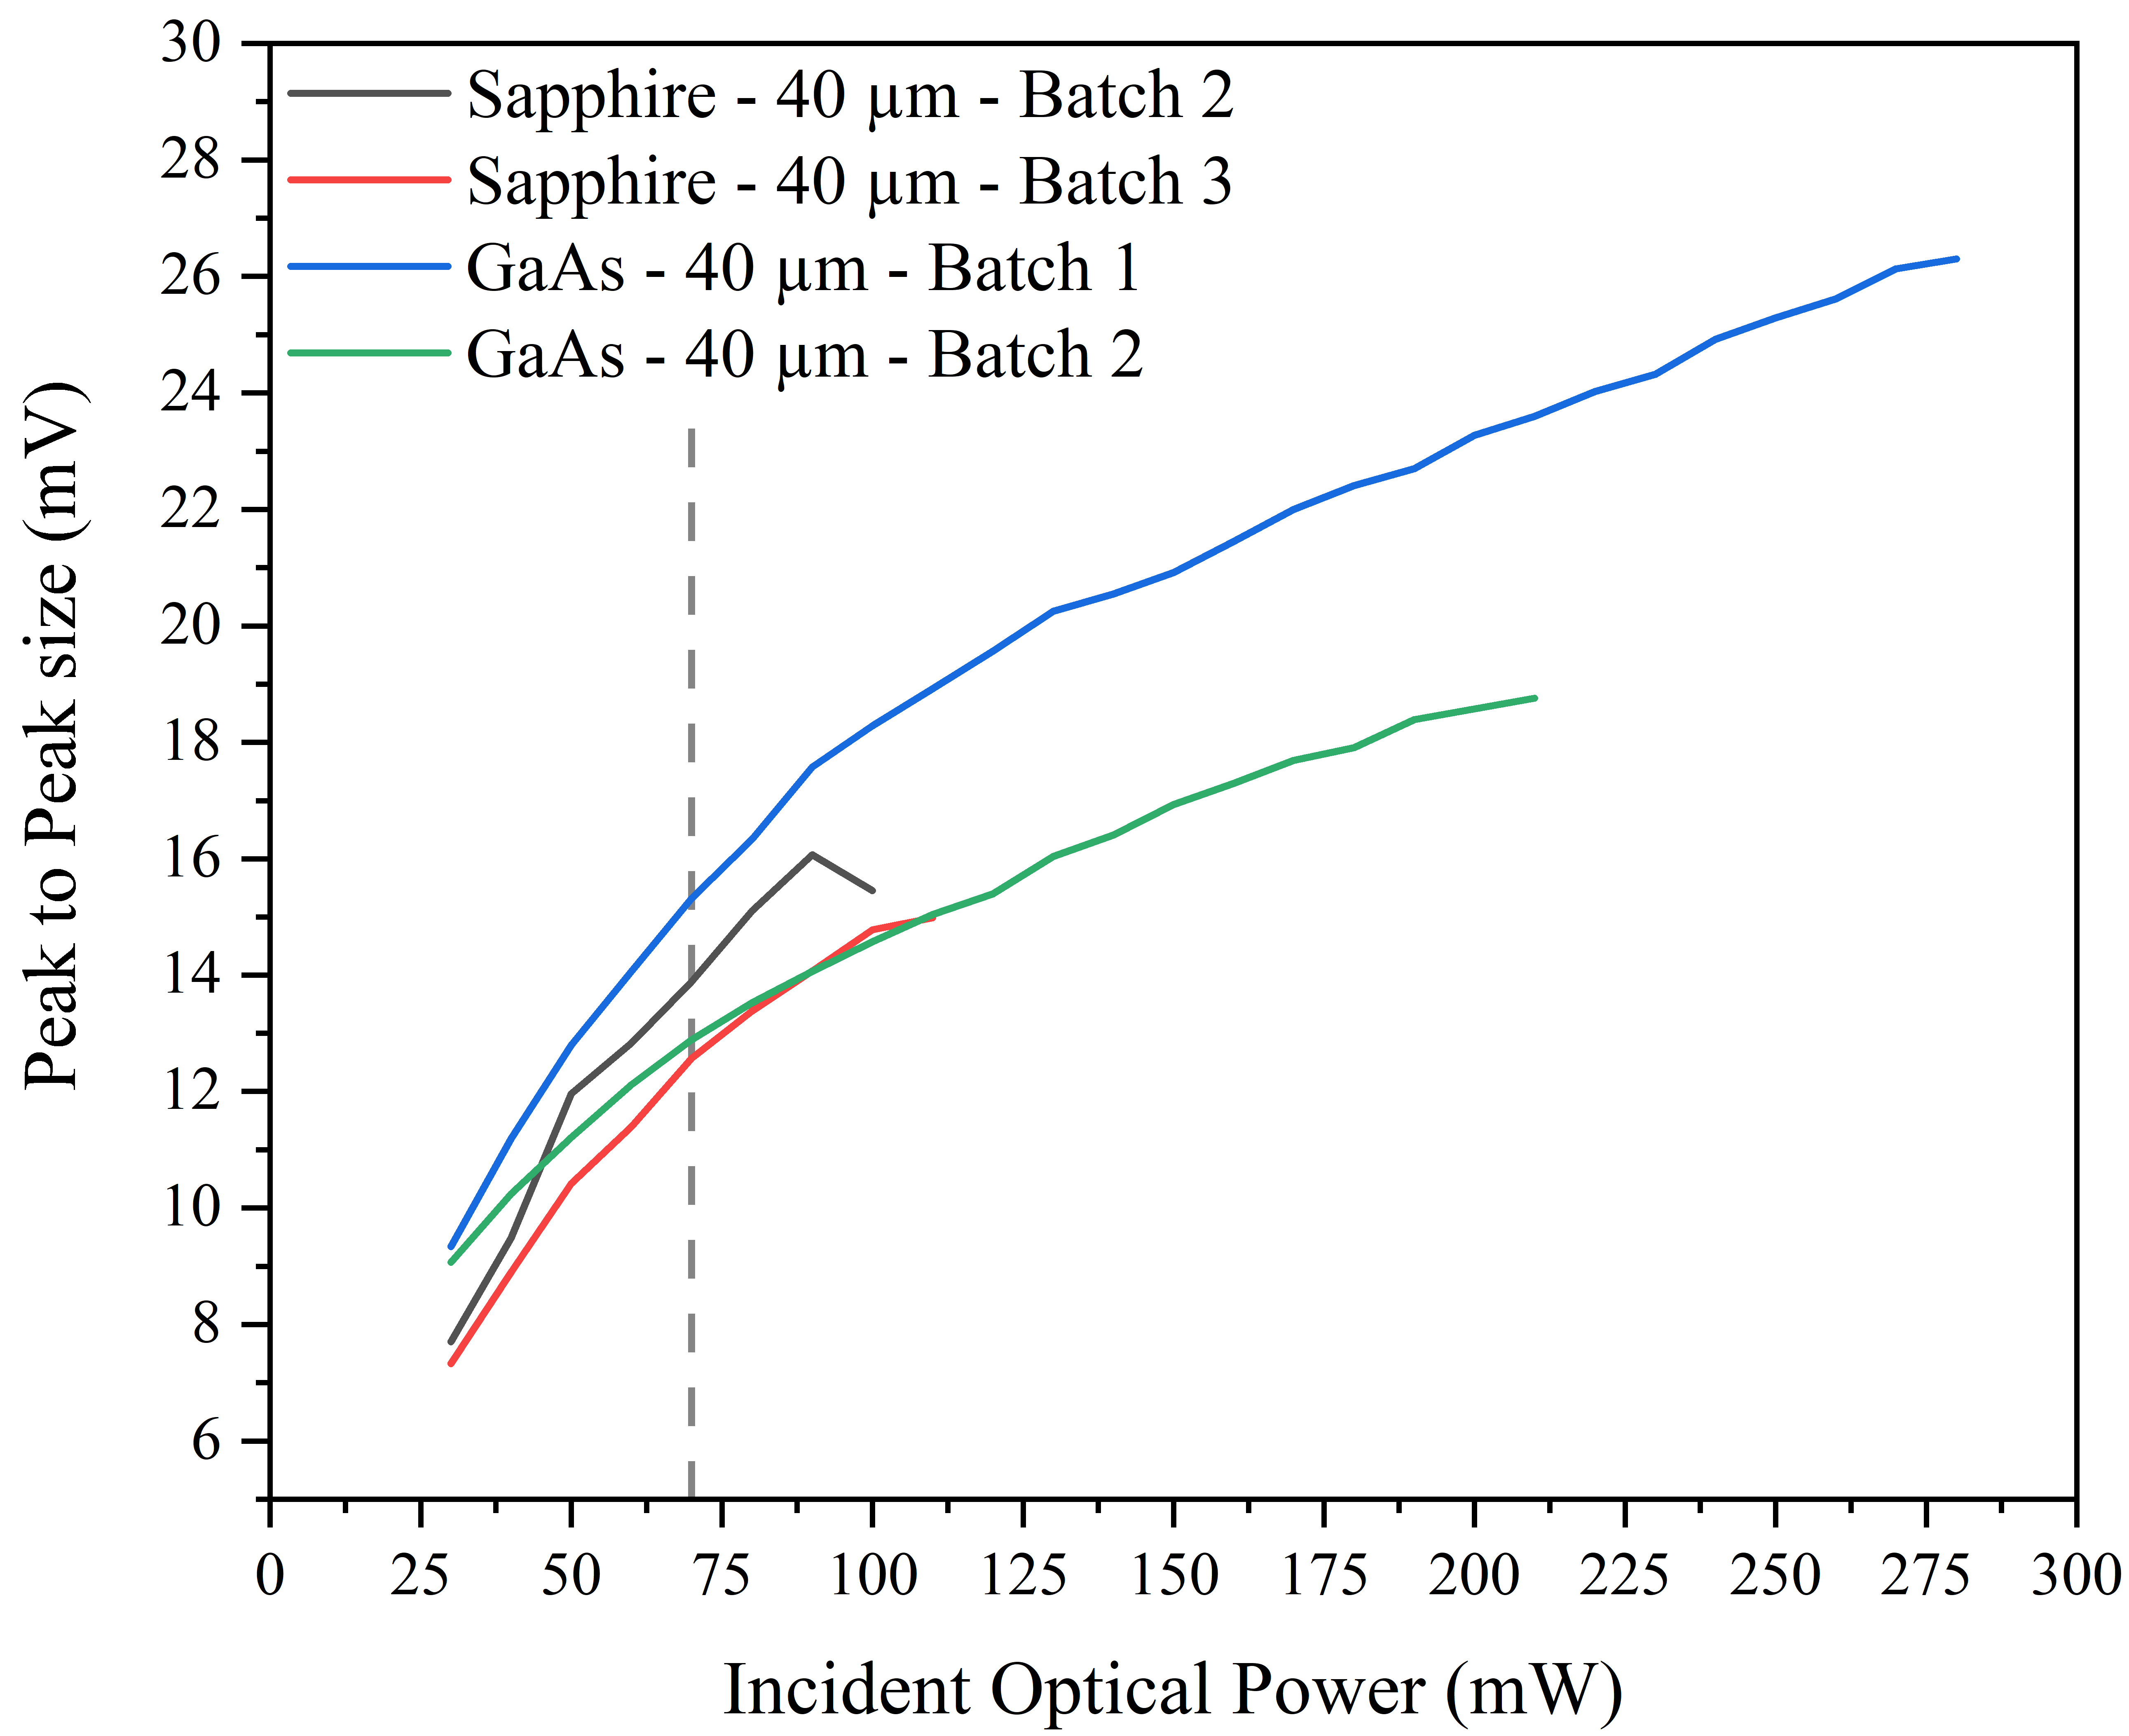
\includegraphics[width=0.6\textwidth]{Figures/Misc/SysDev/Opt40micronG.png}
    \captionsetup{font = footnotesize, justification = centering}
    \caption[The Peak to Peak Signal Values for all Devices with \SI{40}{\micro\metre} Gap]{The peak to peak signal values for all devices with a gap size of \SI{40}{\micro\metre}. The sapphire devices saturate much earlier than expected when compared to their GaAs counterparts.}
    \label{fig:s40micron}
\end{figure}

All the results from devices fabricated using a sapphire substrate are shown in \Cref{fig:allsapph}. There is some significant disagreement between batches, particularly when considering the \SI{10}{\micro\metre} devices but this is presumed to be fabrication issues with the substrate transfer owing to the consistent saturation behaviour within batches. From the trends available it seems that competing factors such as alignment, saturation tolerance and generation efficiency result in the 10 and \SI{40}{\micro\metre} devices producing a similar output for an incident optical power of \SI{70}{\milli\watt} but the device from Batch~2 disagrees with this trend, being one of the best performing devices. Whilst there are inconsistencies, it would seem that \SI{20}{\micro\metre} is the desired gap size for balancing the practicalities of alignment with the maximum power output and desired saturation power.

\begin{figure}[h!]
    \centering
    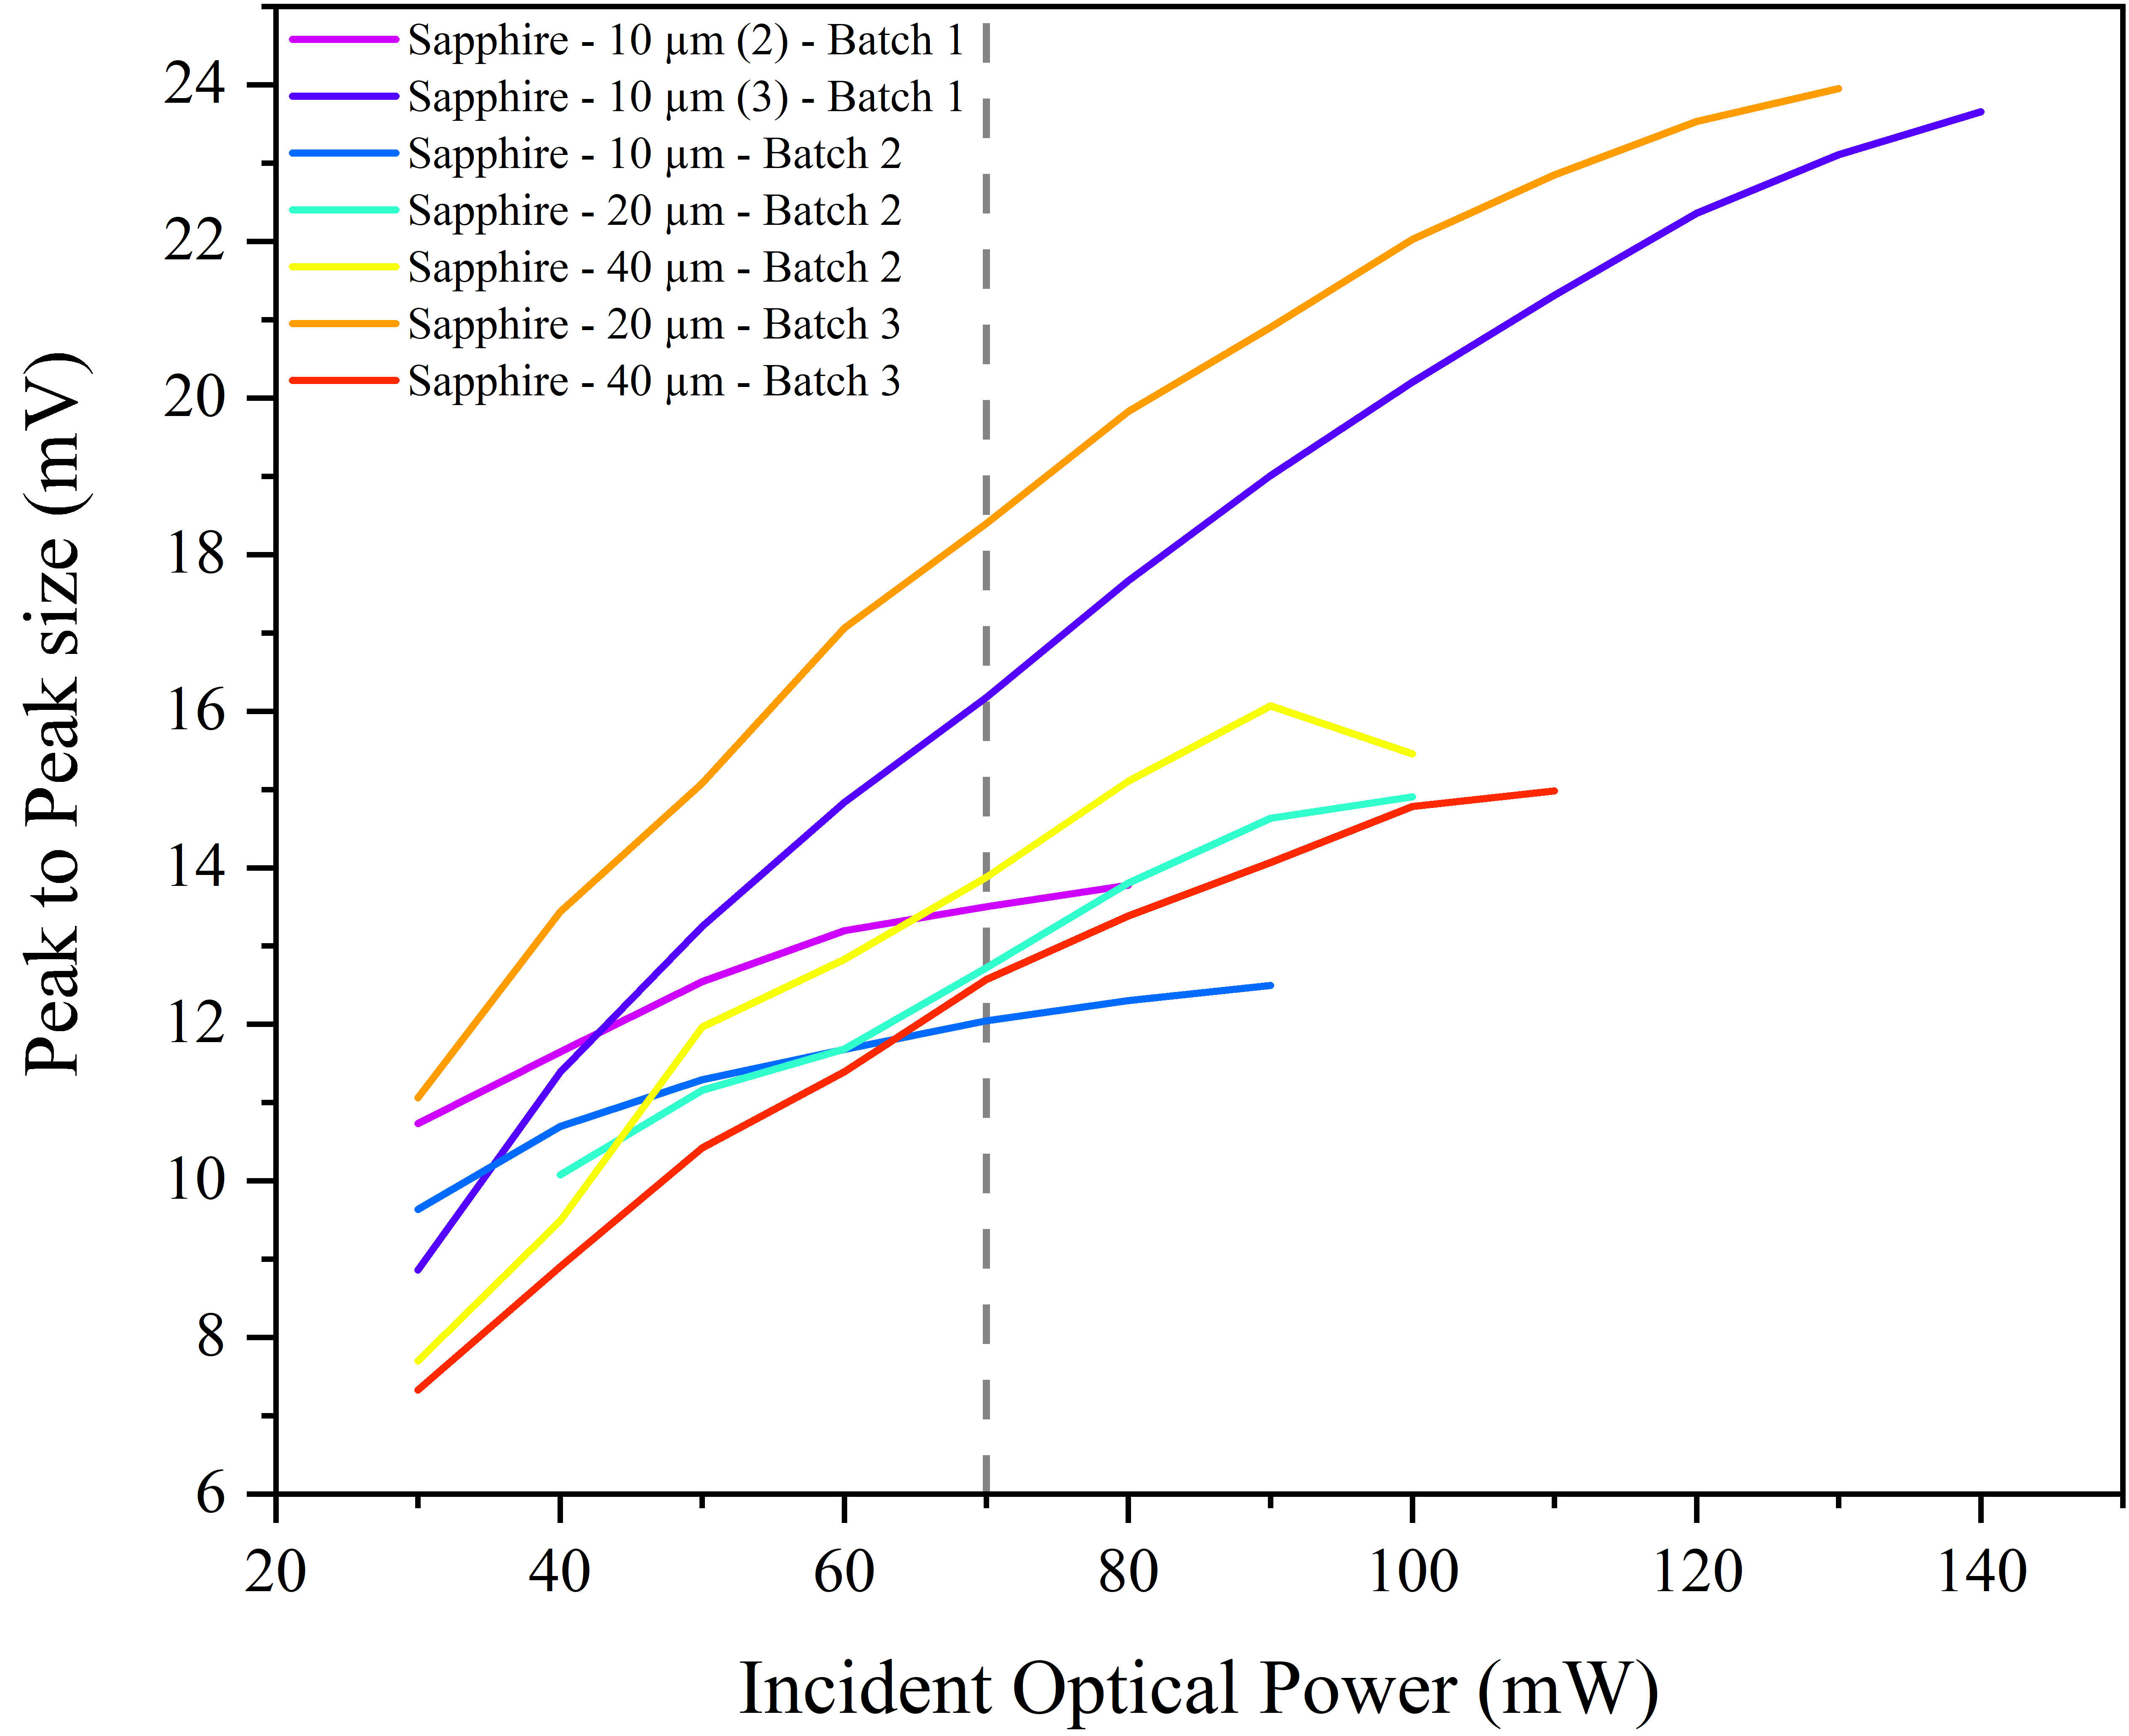
\includegraphics[width=0.8\textwidth]{Figures/Misc/SysDev/OptSapphAllG.png}
    \captionsetup{font = footnotesize, justification = centering}
    \caption[The Peak to Peak Signal Values for all Sapphire Substrate Devices]{The peak to peak signal values for all Sapphire substrate devices. There are some discrepancies between and within batches but the most desirable device is the \SI{20}{\micro\metre} device from Sapphire Batch~2 which has the highest output for the sapphire devices.}
    \label{fig:allsapph}
\end{figure}

\Cref{fig:pcdeviceexamplepic} shows pictures of three example \SI{20}{\micro\metre} devices on sapphire substrates. The pictures show the same three devices but at two different views for clarity. These devices were fabricated in one batch and so should be nominally identical but it is evident that this is not the case. The degree to which the electrodes stick to the surface varies significantly, most critically across the raised edge where the \acrshort{lt}\nobreakdash-GaAs begins. This edge is one area that can be vulnerable to damage when a large photocurrent flows through it which is worsened with inconsistencies in electrode thickness and defects along this edge. This can be clearly seen on the middle and right devices and so it is expected that these would saturate before the device on the left. It is likely that this issue was partially responsible for inconsistencies between and within nominally identical batches.

\begin{figure}[h!]
\centering
\begin{subfigure}{1\textwidth}
    \centering
    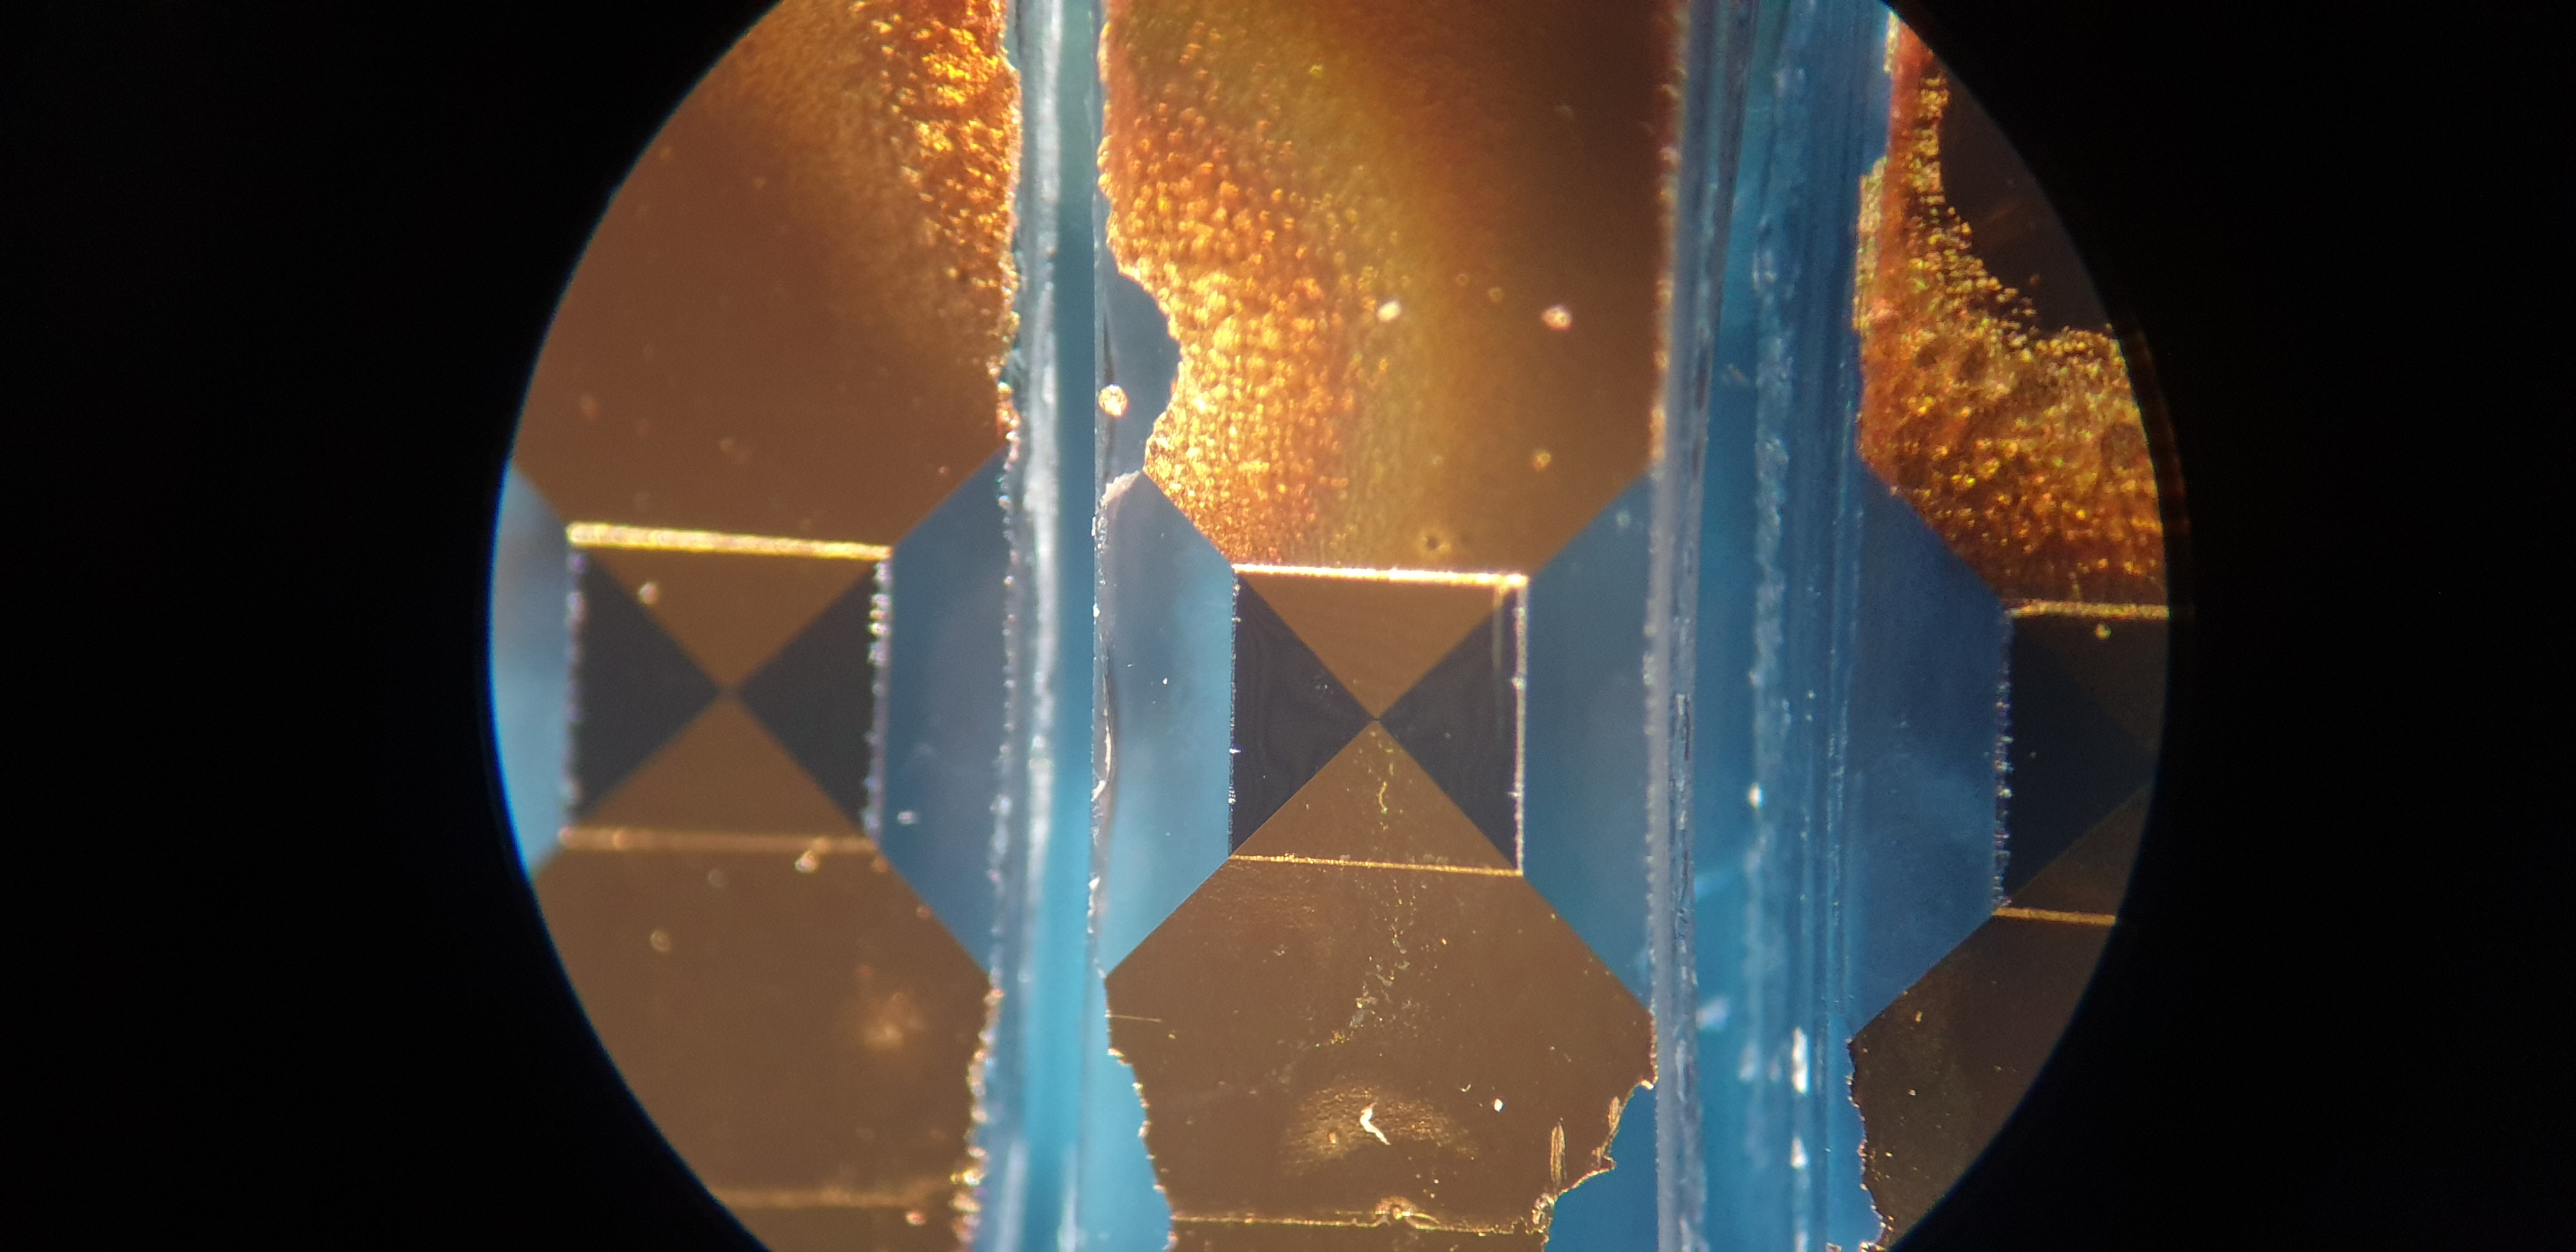
\includegraphics[scale=0.07]{Figures/Misc/SysDev/20220428_104202.jpg}
    \caption{Pic 1}
    \label{fig:devicepic1}
\end{subfigure}
\begin{subfigure}{1\textwidth}
    \centering
    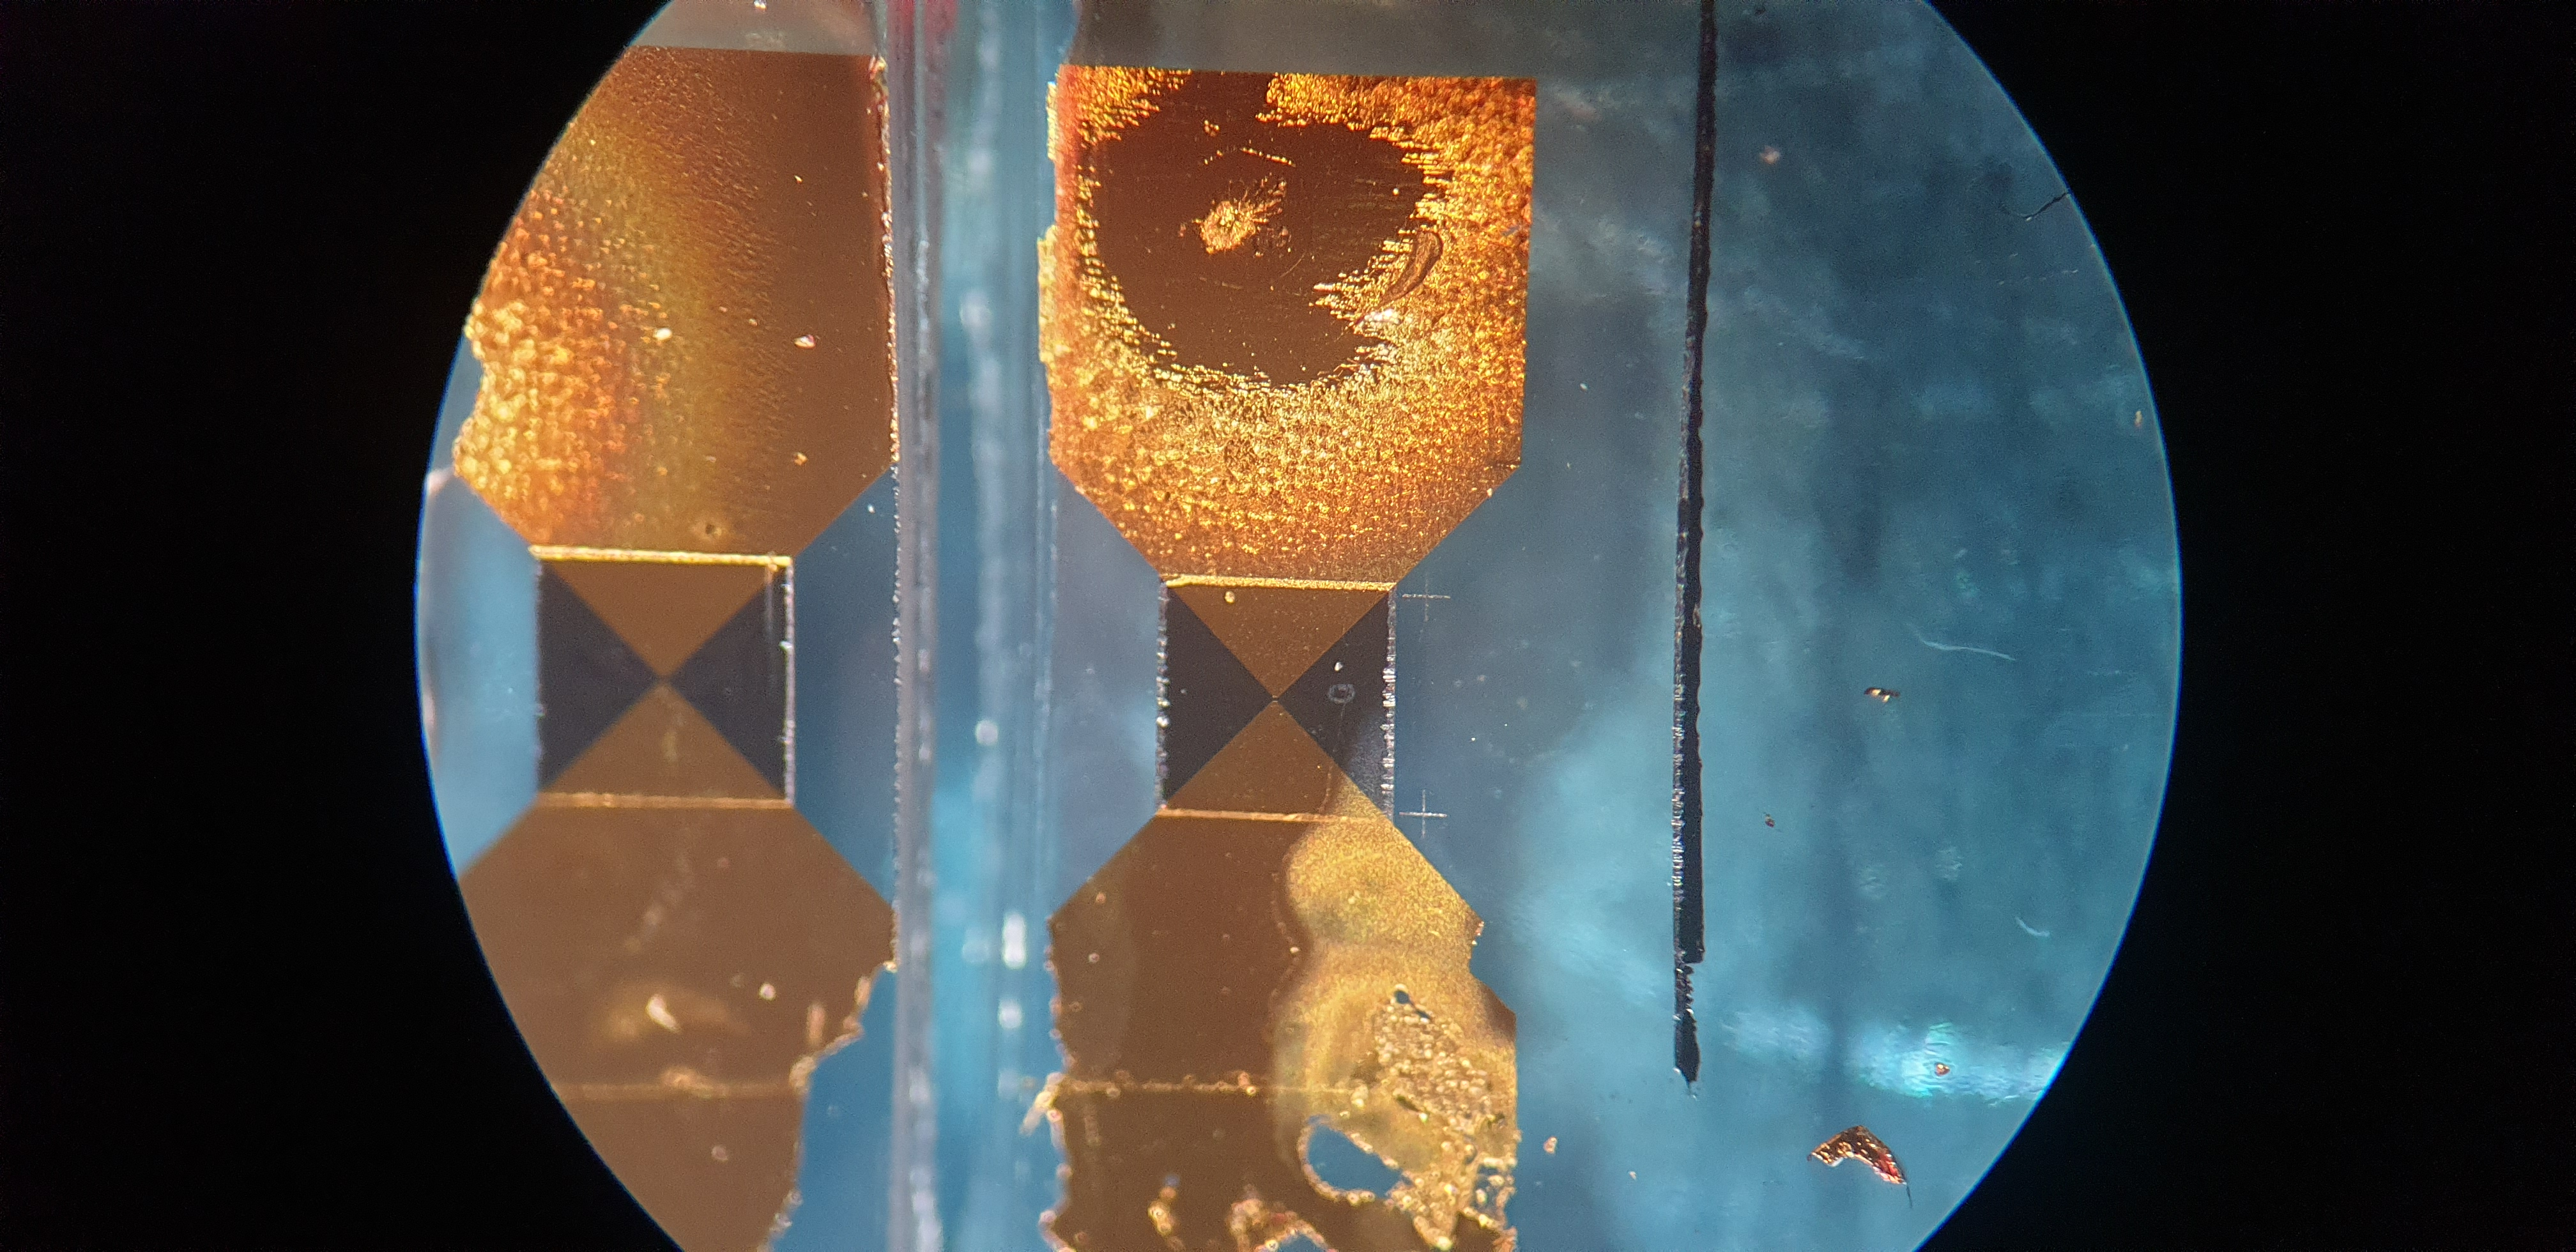
\includegraphics[scale=0.07]{Figures/Misc/SysDev/20220428_104216.jpg}
    \caption{Pic 2}
    \label{fig:devicepic2}
\end{subfigure}
\captionsetup{font = footnotesize, justification = centering}
\caption[Pictures of LT-GaAs on Sapphire Substrate Devices]{Pictures of \acrshort{lt}\nobreakdash-GaAs on Sapphire substrate devices to demonstrate inconsistency in electrode coating. These devices were fabricated in one batch and so should be nominally identical but it is evident that this is not the case.}
\label{fig:pcdeviceexamplepic}
\end{figure}

\section{Emitter Testing with Fibre Laser}
\label{sec:fibrelaser}
Once the \SI{20}{\micro\metre} device had been selected as the optimal choice, this was then incorporated into System~3 that uses the Toptica Fibre laser. This system is still under construction and is subject to change, but the initial set\nobreakdash-up used a \SI{2}{mm} ZnTe \acrshort{eo} crystal as a detector and applied biases were modulated using a \SI{7}{kHz} square wave for lock\nobreakdash-in detection. A series of tests were performed on the selected device in the emitter position where the optical power hitting the emitter and the \acrshort{eo} detector were varied respectively, along with the bias applied to the emitter and the rotation of the \acrshort{eo} crystal in its mount. The results of these tests is shown in \Cref{Fig:fiblaser}

\begin{figure}[ht]
\centering

\begin{subfigure}{0.49\textwidth}
\centering
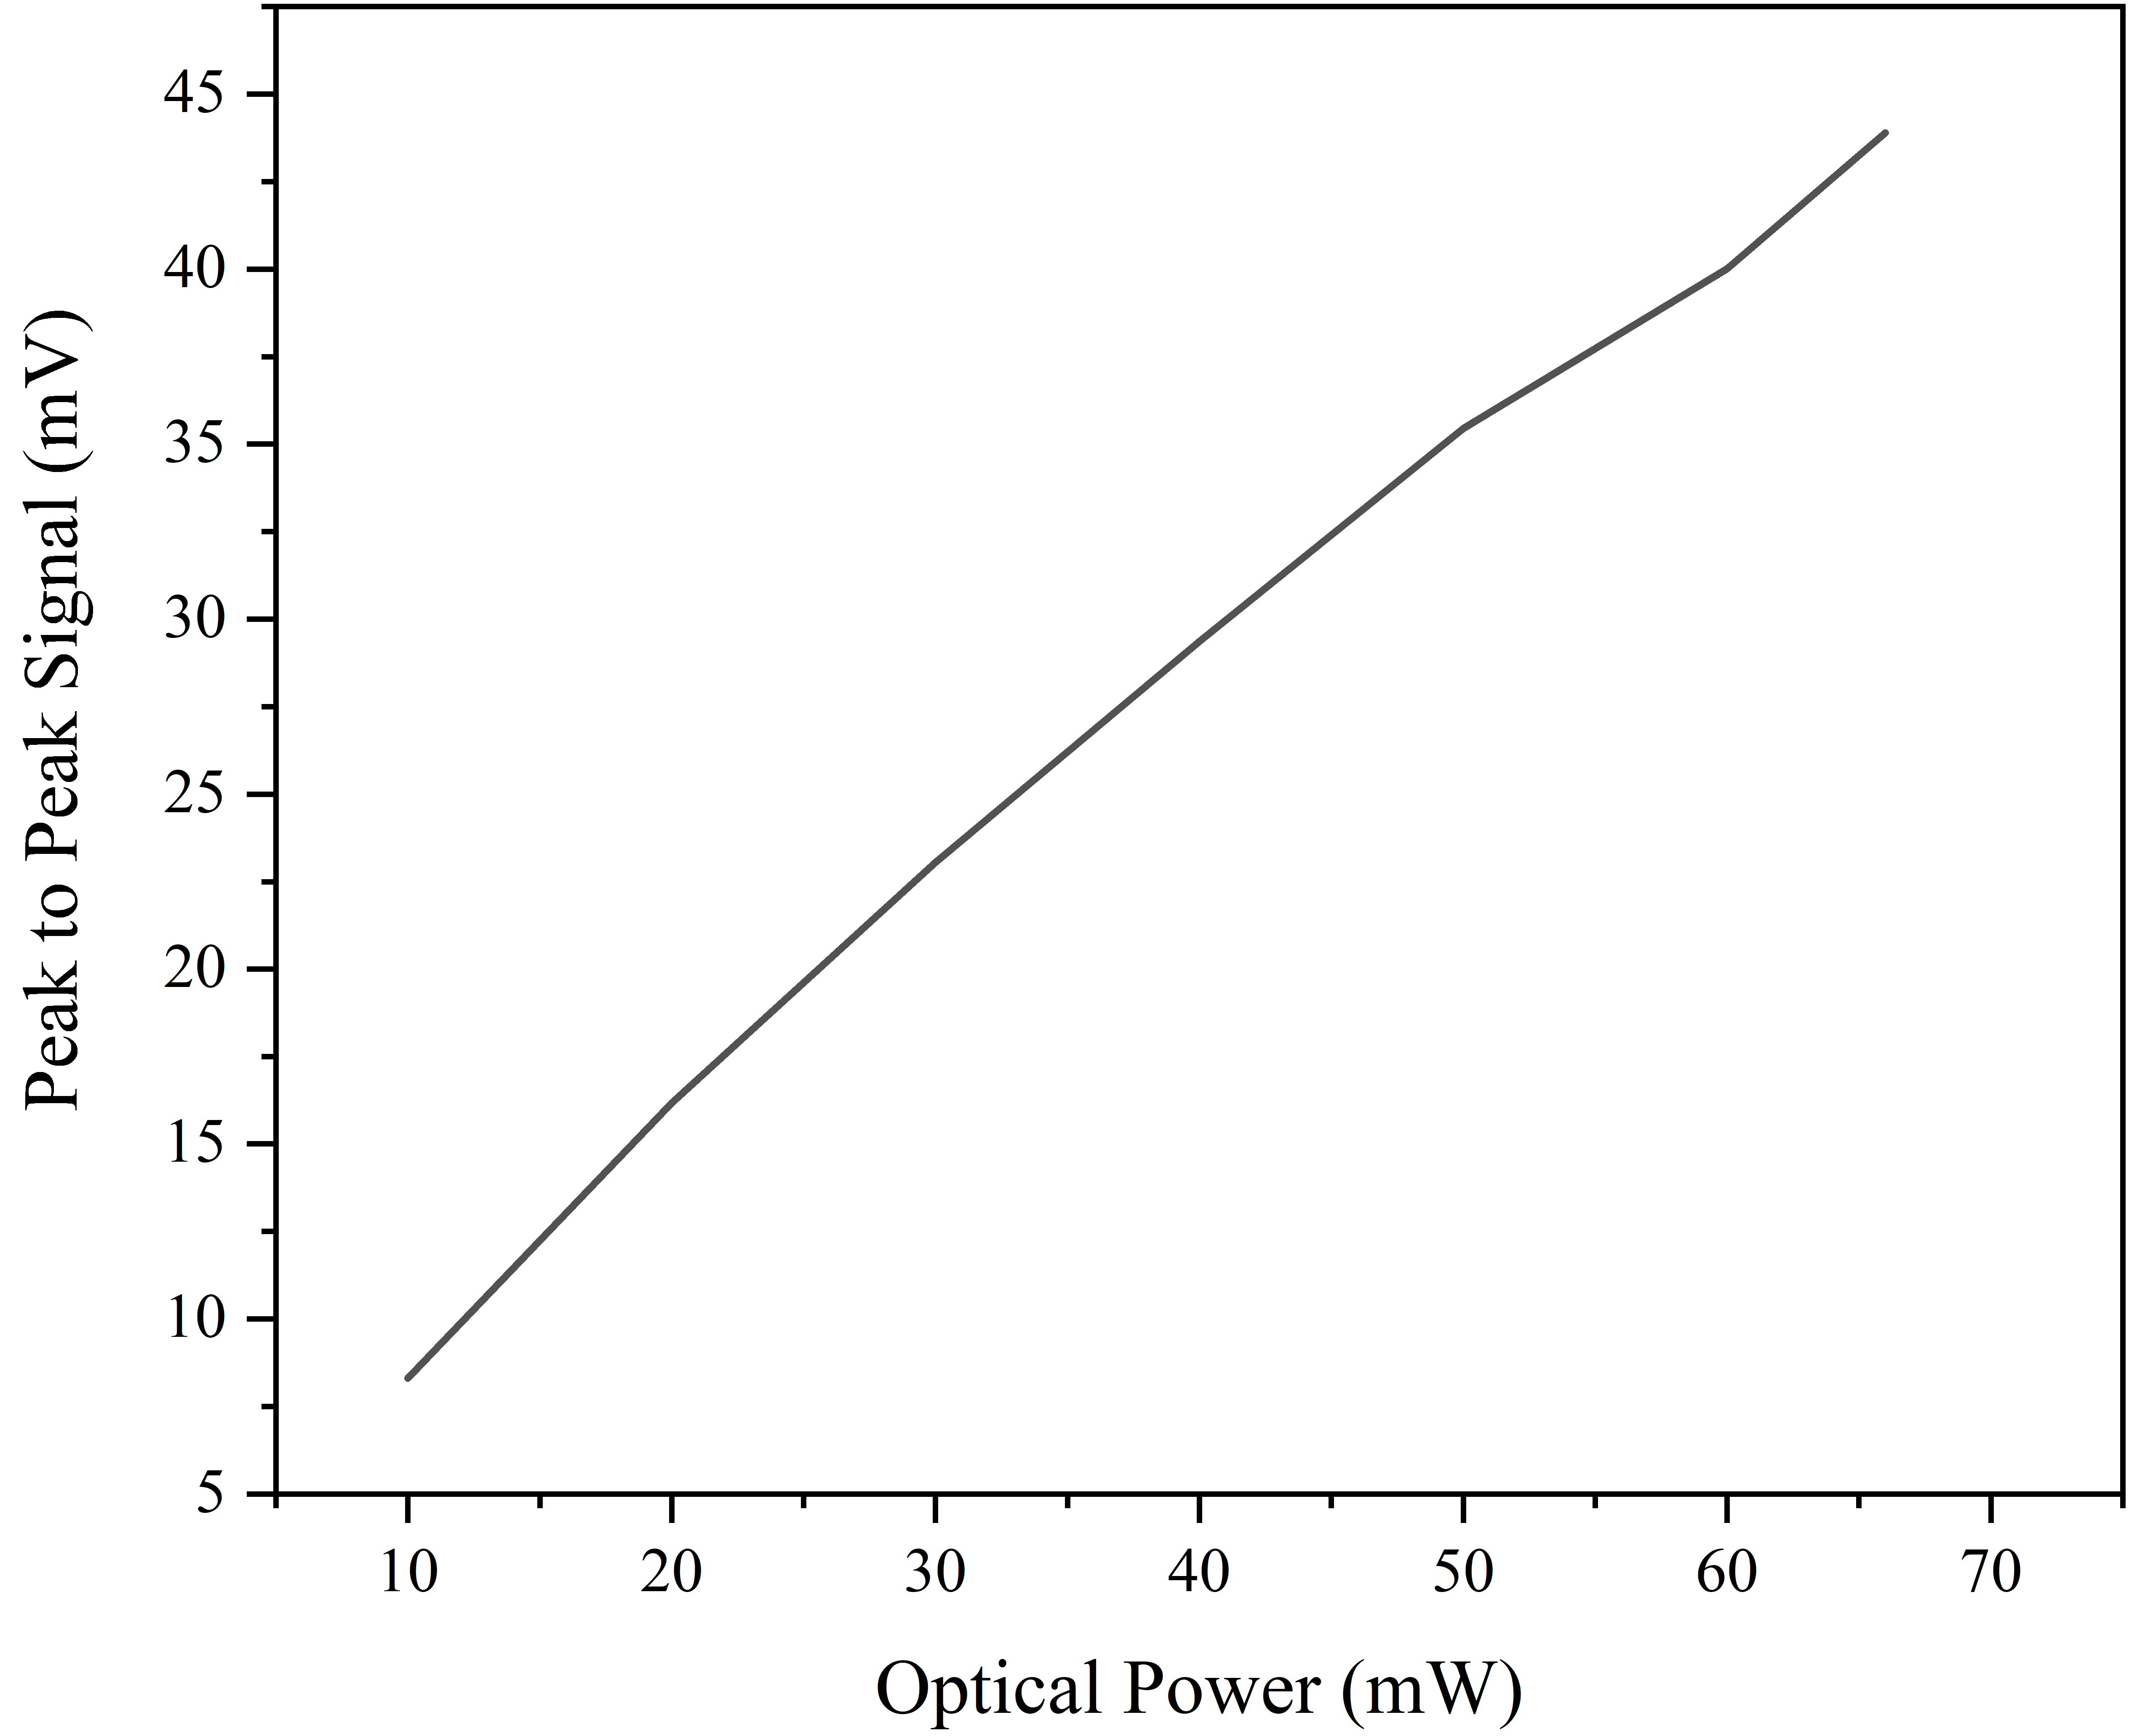
\includegraphics[width=\textwidth]{Figures/Misc/SysDev/NBOpt150VG_V2.png}
\caption{Optical Sweep - Emitter}
\label{fig:NBOpt150V}
\end{subfigure}
\begin{subfigure}{0.49\textwidth}
\centering
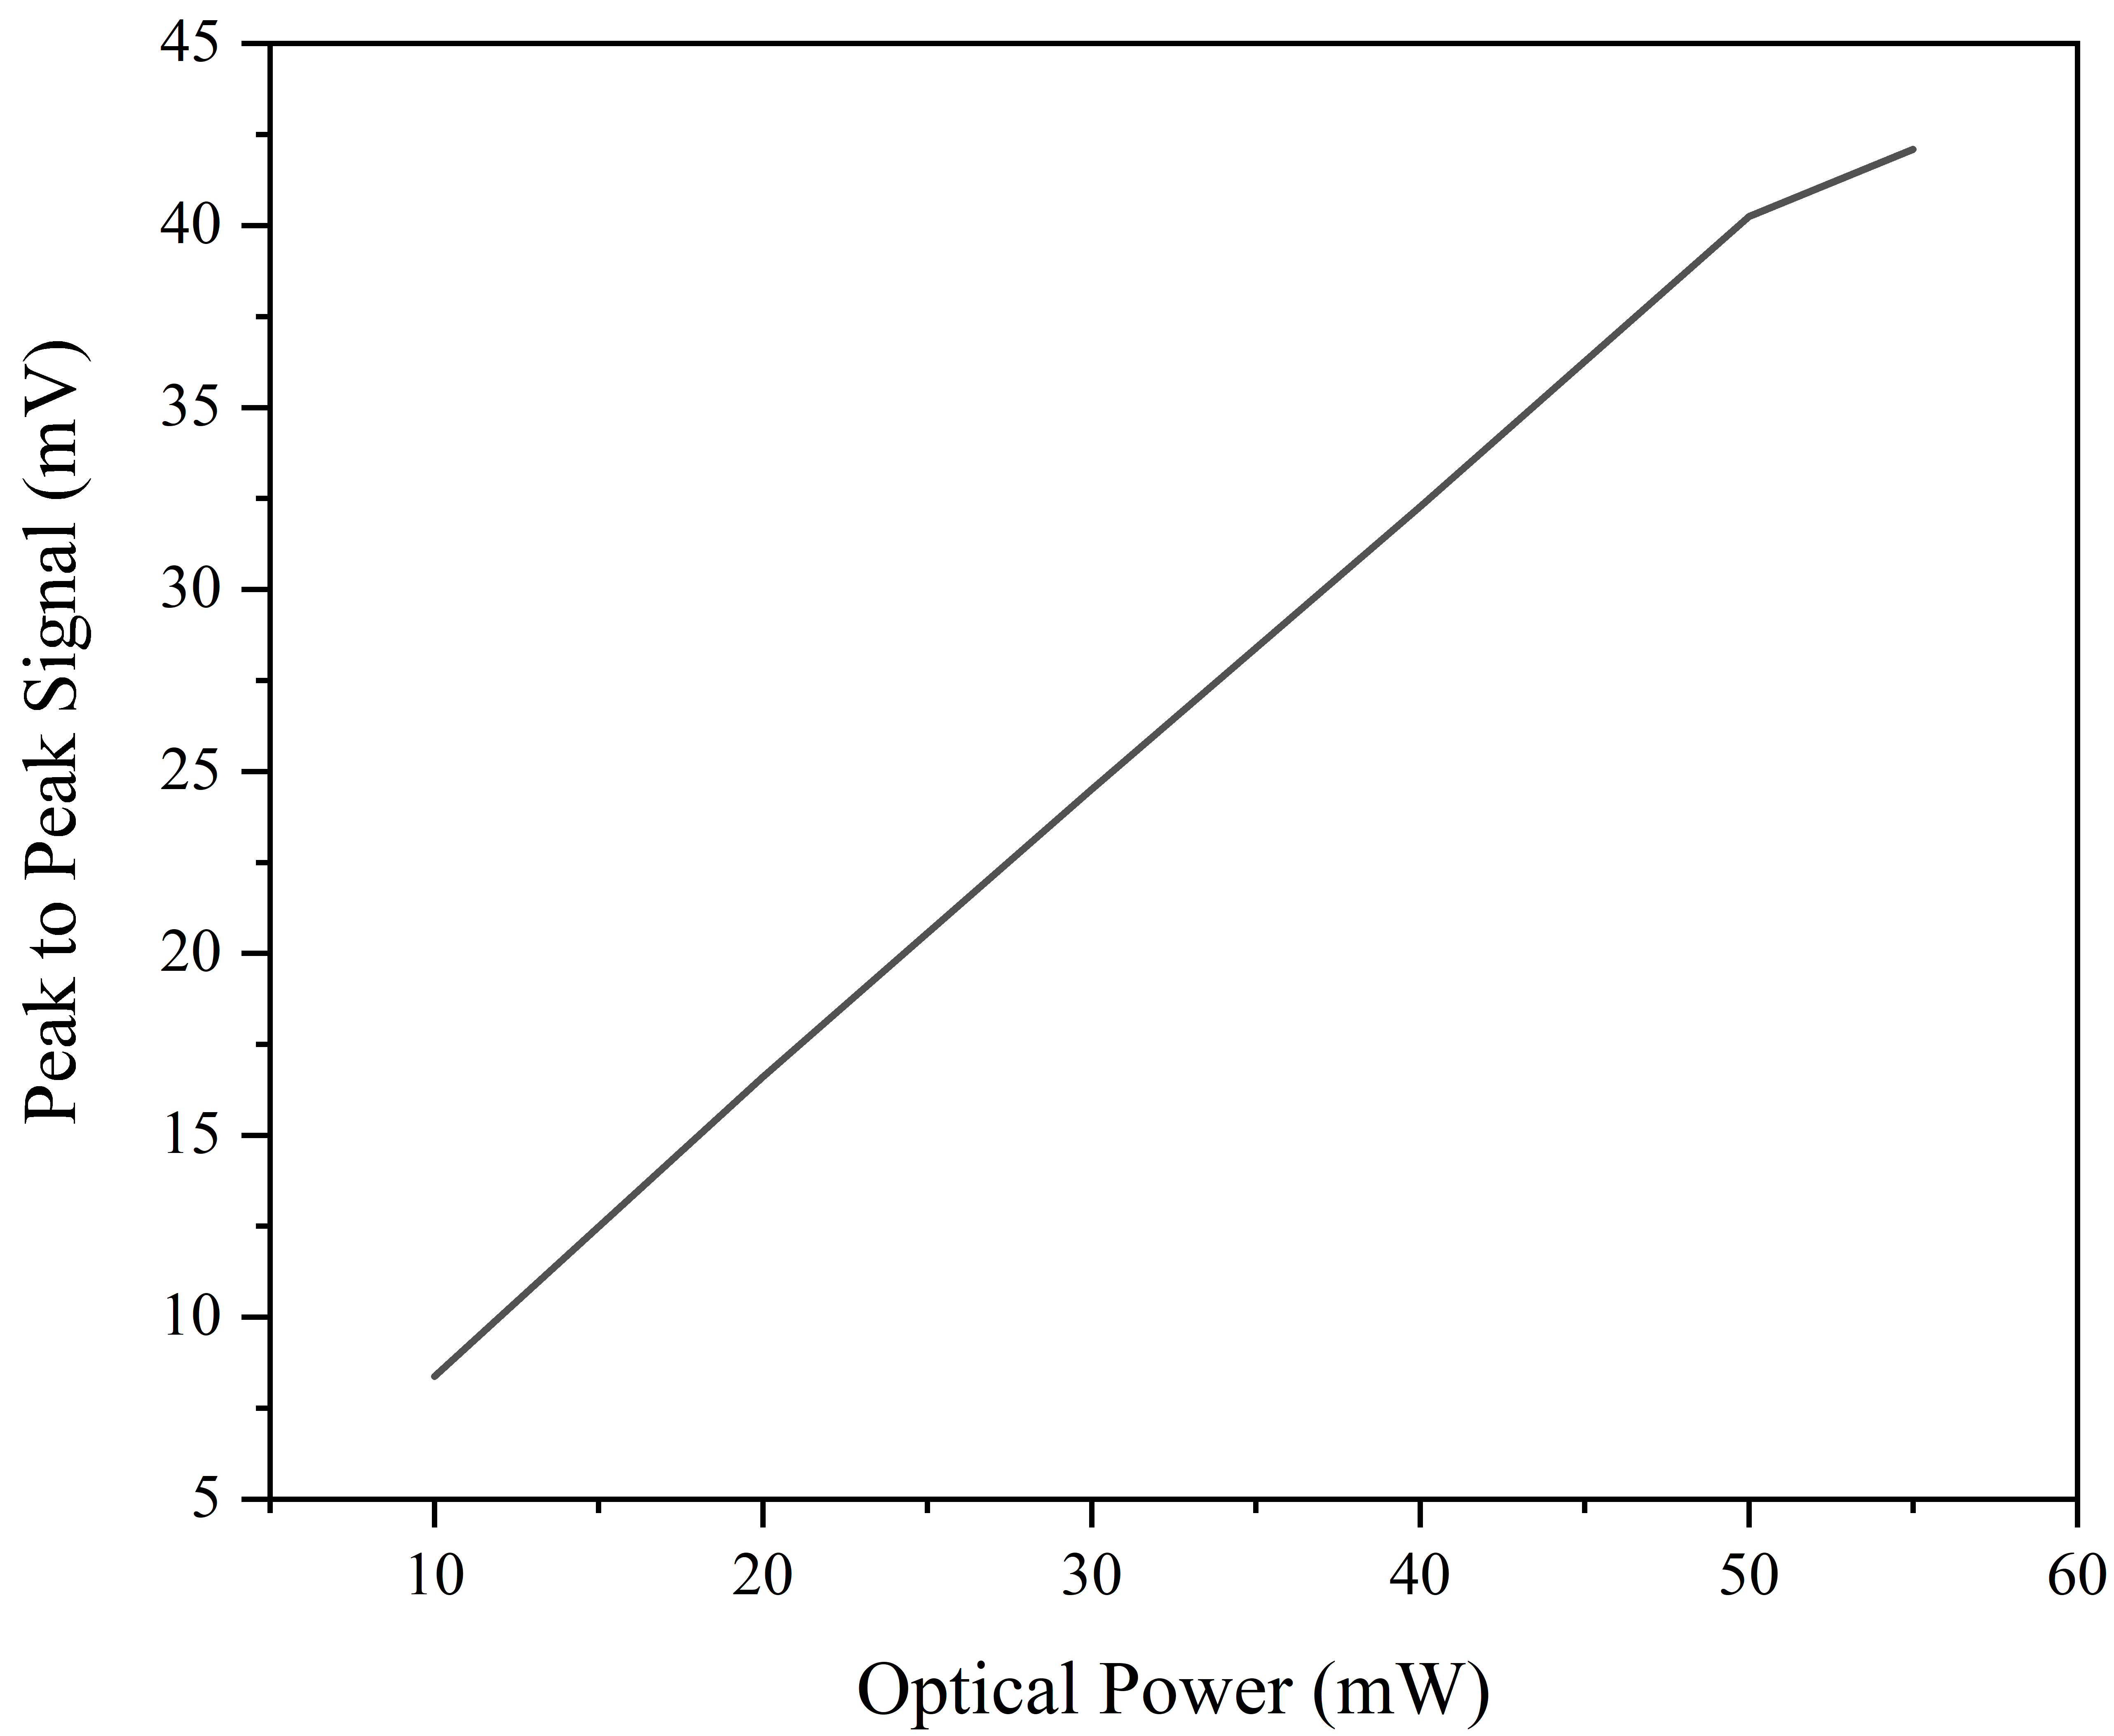
\includegraphics[width=\textwidth]{Figures/Misc/SysDev/NBOptDet150V_V2.png}
\caption{Optical Sweep - Detector}
\label{fig:NBOptDet150V}
\end{subfigure}

\begin{subfigure}{0.49\textwidth}
\centering
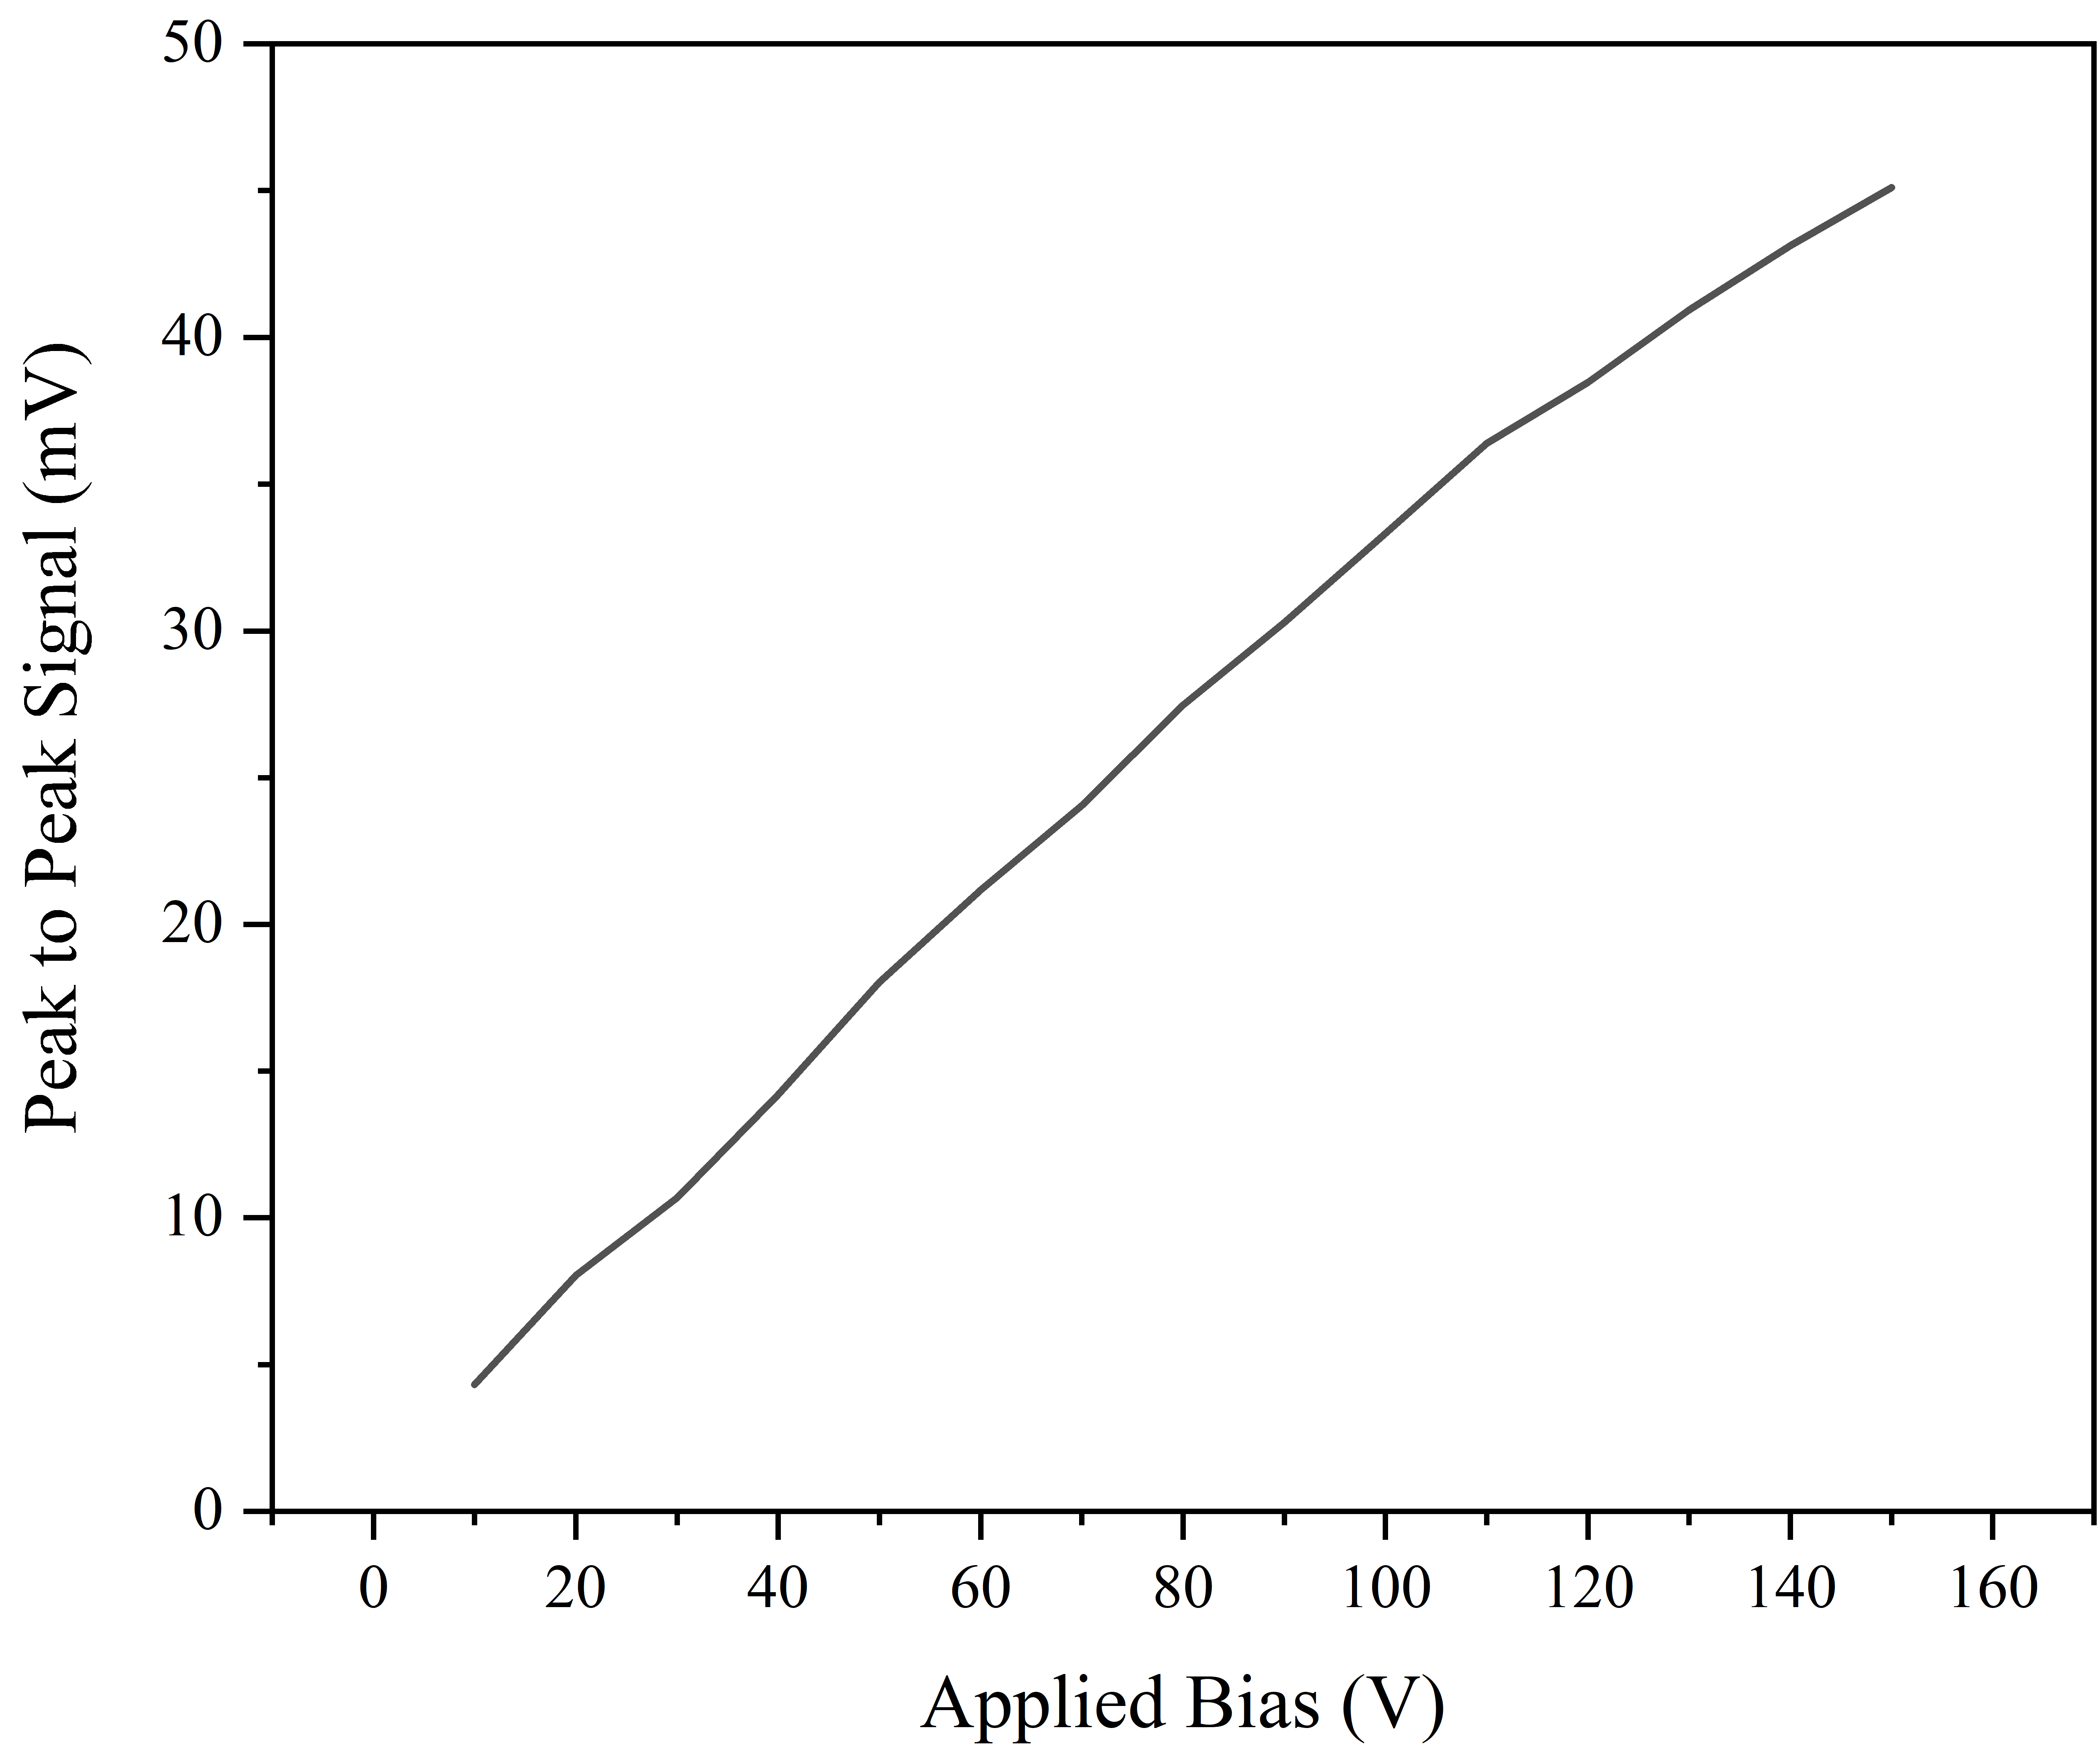
\includegraphics[width=\textwidth]{Figures/Misc/SysDev/NBVoltE63G.png}
\caption{Voltage Sweep - Detector}
\label{fig:NBVoltE63G}
\end{subfigure}
\begin{subfigure}{0.49\textwidth}
\centering
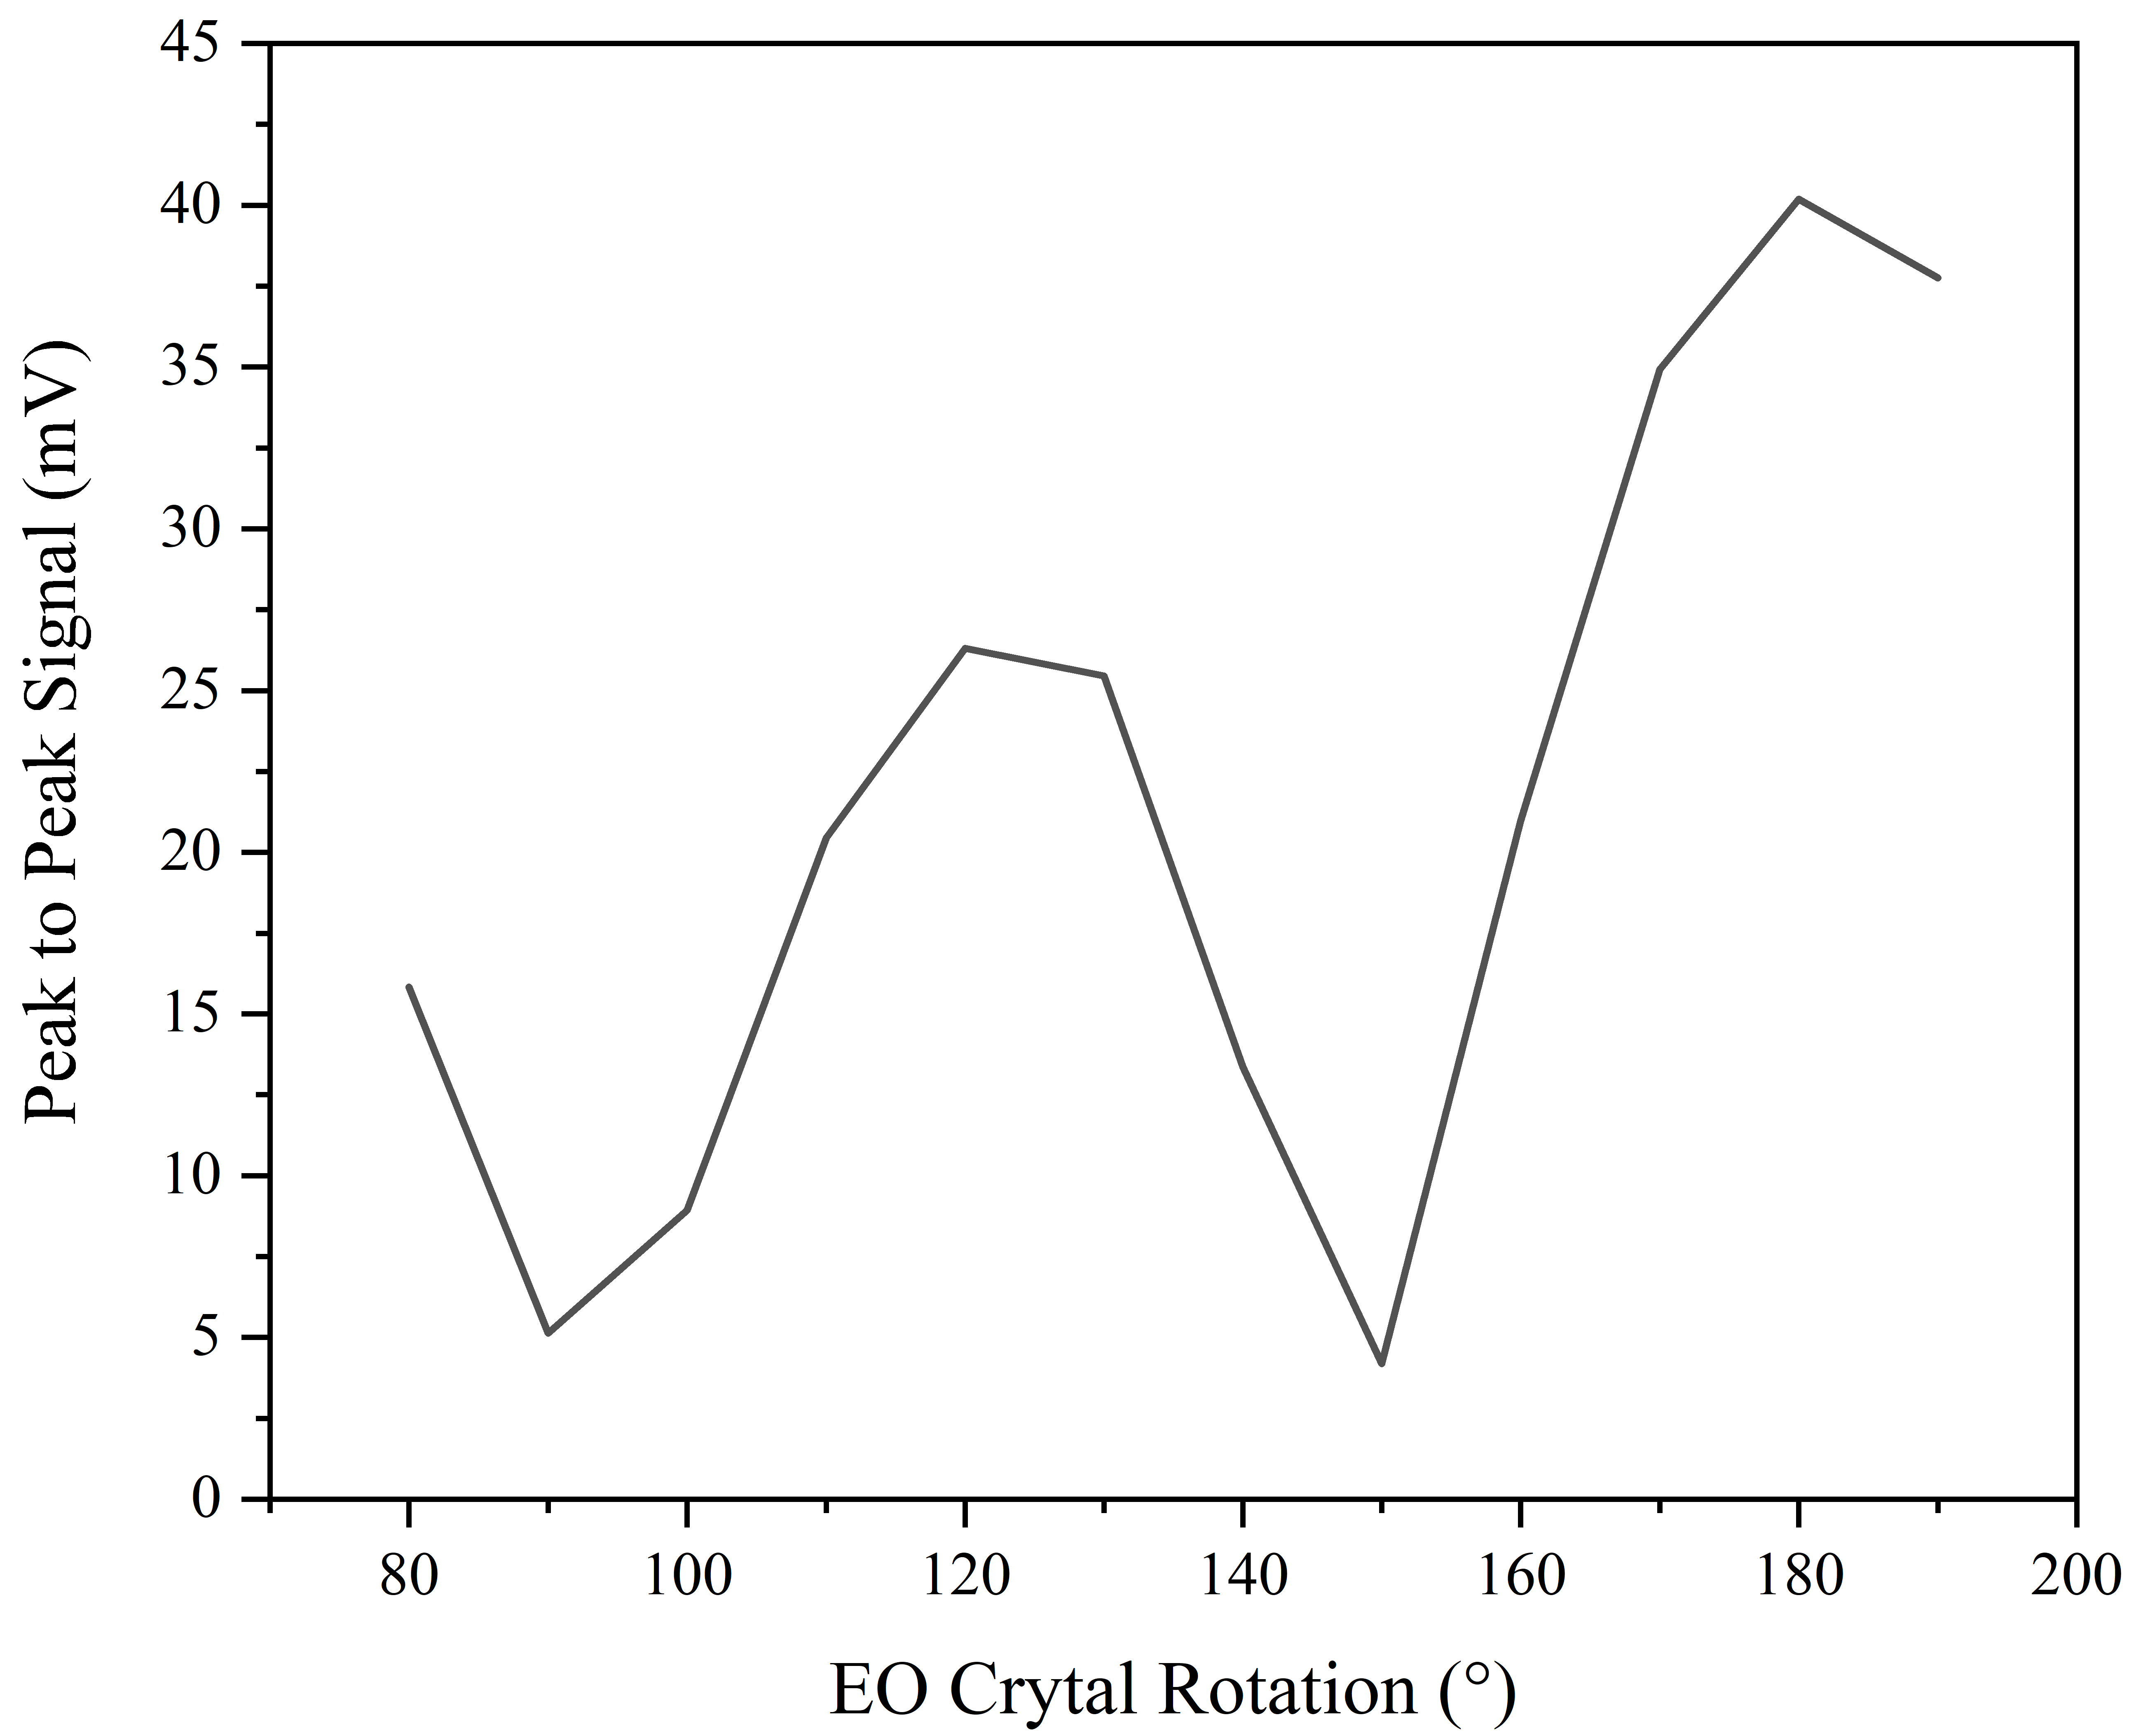
\includegraphics[width=\textwidth]{Figures/Misc/SysDev/A20umEORotG.png}
\caption{Rotation of EO Crystal}
\label{fig:A20umEORotG}
\end{subfigure}

\captionsetup{font = footnotesize, justification = centering}
\caption[Testing of a \SI{20}{\micro\metre} Device on a Sapphire Substrate using the Fibre Laser]{Testing of a \SI{20}{\micro\metre} device on a sapphire substrate using the fibre laser in System~3.}
\label{Fig:fiblaser}
\end{figure}

The \acrshort{eo} crystal's rotation was performed first and a clear maximum can be seen at \ang{180}. This is shown in \Cref{fig:A20umEORotG} and \ang{180} was used for all remaining scans. The variation of the incident optical power on the emitter is shown in \Cref{fig:NBOpt150V} and the device appears to be beginning to saturate but more optical power would be required to confirm this. The saturation behavior is easier to see in \Cref{fig:NBOptDet150V} but this is from a different mechanism in the \acrshort{eo} crystal. Both these tests were performed using the maximum incident power on the emitter or detector respectively and an applied bias of \SI{150}{V}. Finally, the applied bias was varied while the maximum incident power was directed to both the emitter and detector. The device begins to saturate at around 140--\SI{150}{V} which is reasonable. Whilst the saturation behaviour of the \SI{20}{\micro\metre} device is not completely ideal, it seems the clear choice for use at the incident optical powers that System~3 will utilise, owing to it being relatively easy to align whilst producing a desirable output. 

\section{Conclusion}
This chapter described the investigation into the effect of gap\nobreakdash-size on the output of \acrshort{pc} switches, specifically at the relatively low optical power ranges that will be utilised by System~3 which is under construction. Devices with both sapphire and GaAs substrates were tested owing to the significantly easier alignment of GaAs devices and to confirm the results of the sapphire devices. Once an optimal gap size had been selected, the device was tested in System~3 to determine its suitability.

The investigation into gap sizes produced some unexpected results whereby some GaAs devices would outperform their sapphire counterparts. This was attributed to issues with the far more complicated fabrication process, specifically the transfer of the \acrshort{lt}\nobreakdash-GaAs to the sapphire substrate and the application of the Au electrodes. However, System~3 will require an emitter and detector with optically transparent substrates so this slight improvement in performance has not been considered. It was determined that the 5 and \SI{10}{\micro\metre} devices were too difficult to align and were not chosen. As the \SI{20}{\micro\metre} device performed better than the \SI{40}{\micro\metre} device, this was selected as the optimal size.

A \SI{20}{\micro\metre} device was put into System~3 as an emitter and a ZnTe crystal was used as preliminary detector. The device performed satisfactorily when both the incident optical power and the applied bias was varied and the optimal parameters for the ZnTe crystal were selected. This project was significantly hampered by the pandemic whereby the multiple, lengthy closures and subsequent occupancy rules of the laboratory prevented any meaningful progress for a significant portion of the time available. Additionally, the fibre laser in System~3 required repairing and was unavailable for a number of months.


